

%----------------------------------------------------------------------------------------
%	PART
%----------------------------------------------------------------------------------------




\part{Ejercicios}
\graphicspath{ {img/tablas/}, {img/} }

%----------------------------------------------------------------------------------------
%	Ejercicios
%----------------------------------------------------------------------------------------

\chapterimage{ima2} % Chapter heading image

\chapter {Ejercicios}

\chapter*{Capítulo 1}
\addcontentsline{toc}{chapter}{\textcolor{ocre}{Capítulo 1}}


\begin{itemize}
	\item 1. Calcular el interés simple (I, en pesos) comercial de \$300.000 desde el 18 de marzo al 18 de junio del mismo año al 3,4\% periódico mes vencido.\\
	\textbf{Respuesta:} \$30.600
	\medskip
	
	\item 2. Una persona invierte \$250.000 al 40\% EA desde el 15 de septiembre de 1998 hasta el 18 de noviembre de 1998. Calcular: 
	\\
	a) el valor final racional y
	b) el valor final bancario. 
	\\
	\textbf{Respuestas:} a) \$267.534,25  b) \$2'677.777,78
	\medskip
	
	\item 3. ¿Cuánto debe invertirse hoy 17 de octubre en un fondo que garantiza el 28\% EA  real para que el 20 de marzo del siguiente año pueda retirar la suma de \$150.000?\\
	\textbf{Respuesta:} \$134.151,72
	\medskip
	
	
	\item 4. Hallar el valor presente de \$500.000 en 3 y 1/2 años al 3\%pmv\\
	\textbf{Respuesta:} \$221.239 
	\medskip
	
	\item 5. Hace 6 años compré un lote en \$900.000 y hoy se vendió en \$6 millones. Hallar la tasa de interés EA comercial que gané en este negocio.\\
	\textbf{Respuesta: }94,44\% EA
	\medskip
	
	\item 6. ¿Qué tan rentable es un documento que hoy se puede comprar en \$75.000 el cual devolverá al cabo de 3 años la suma de \$330.000?\\
	\textbf{Respuesta: }113,33\% EA
	\medskip
	
	\item 7. Se recibe un préstamo por \$1 millón al 42\% nominal anual año vencido el día 8 de agosto de 1999 con vencimiento el 8 de marzo del 2000. Hallar el valor final del préstamo calculando los intereses (I):\\
	
	a) interés exacto o racional\\
	b) interés comercial o base 360\\
	e) interés bancario\\
	d) interés base 365\\
	Tenga en cuenta que el año 2000 es un año bisiesto\\
	\textbf{ Respuestas:} a) \$1'244.426,23; b) \$1'245.000; e) \$1'248.500; d) \$1'243.945,21
	\medskip
	
	\item 8. Un pagaré con valor presente de \$300 000 emitido el 15 de septiembre de 1999 con plazo de 270 días a una tasa de interés del 30\% nominal anual año vencido.\\
	Hallar el valor futuro y la fecha de vencimiento en:\\
	
	a) interés exacto o racional\\
	b) interés comercial o base 360\\
	c) interés bancario\\
	d) interés base 365\\
	\textbf{Respuestas:} a) \$366.393,44; 11-06-00; b) \$367.500; 15-06-00; c) \$367.500; 11-06-00; d) \$366.575,34; 12-06-00
	\medskip
	
	\item 9. Una letra por \$550.000 madura el 23 de agosto de 1998 y va a ser descontada el 17 de julio del mismo año al 38\% EA. Determinar el valor de la transacción.\\
	\textbf{Respuesta:} \$528.519,44
	\medskip
	
	\item 10. El 15 de diciembre de 1999 una empresa recibe un pagaré por \$2 millones a un plazo de 3 meses al 25\% nominal anual año vencido de interés comercial simple. El 14 de enero lo negocia con un banco que lo adquiere a una tasa de descuento del 29\% nominal anual año anticipado en interés bancario. ¿Cuánto recibirá la empresa por el pagaré y cuánto ganará el banco en la operación de descuento?\\
	
	\textbf{Respuestas:} la empresa recibe \$2.020.579,86; el banco gana \$104.420,14
	\medskip
	
	\item 11. Halle el valor de maduración de un pagaré con vencimiento el 20 de abril si va a ser descontado el 13 de marzo del mismo año al 40\% EA y su valor de transacción es de \$ 78.400\\
	\textbf{Respuesta:} \$81.856,15
	\medskip
	
	\item 12. Una persona solicita un préstamo a un banco por la suma de \$800.000, a un plazo de 90 días y le cobran una tasa anticipada del 38\% EA.\\
	
	a) ¿Cuál es el valor líquido que le entregan?\\
	b) Suponga que el banco cobra \$15 000 por el estudio del crédito, ¿cuál será el valor liquido?\\
	
	\textbf{Respuestas:} a) \$724.000; b) \$709.000
	\medskip
	
	\item 13. ¿Cuál es el valor del documento que queda en poder de un banco, si el prestatario recibe un valor liquido de  \$50.000 por un documento con maduración en 90 días, si le cobran una tasa de descuento del 41\% EA? \\
	
	a) Sin tener en cuenta costos de apertura del crédito y\\
	b) Teniendo en cuenta que el banco cobra \$2 000 por estudio del documento \\
	\textbf{Respuestas:} a) \$55.710,31; b) \$57.938,72
	\medskip
	
	\item 14. Un documento de valor inicial \$70.000 es fechado el 25 de septiembre de 1998 a un plazo de 325 días y un interés del 32\% EA. Si es descontado por un banco el 18 de marzo de 1999 al 40\% EA determinar:\\
	
	a) la fecha de vencimiento\\
	b) El valor al vencimiento\\
	c) El valor de transacción \\
	Usar interés bancario\\
	
	\textbf{Respuestas:} a) 16-08-99; b) \$90.222,22; c) \$75.084,94
	\medskip
	
	\item 15. Hallar la verdadera tasa bancaria que cobra un banco cuando descuenta un documento con valor de maduración de \$400.000 si es descontado 25 días antes del vencimiento al 41\% nominal anual año anticipado.\\
	
	\textbf{Respuesta:} 42,2\% nominal anual año vencido
	
	\item 16. Un almacén ofrece los siguientes descuentos, sobre una mercancía cuyo costo inicial es de \$200.000:\\
	
	30\% por venta al por mayor, 10\% por pago al contado y 5\% por enviar la mercancía sin empaque.\\
	
	a)¿Cuál es el valor final de la factura?\\
	b) ¿Cuál es el descuento promedio que se otorgó?\\
	
	\textbf{Respuestas:} a) \$119.700 b) 40,15\%
	
	\item 17. Una fábrica ofrece un descuento del 25\% en ventas al por mayor, el 5\% por pronto pago y el 4\% por embalaje. ¿Cuál debe ser el descuento adicional que puede ofrecerse a los empleados de la misma fábrica para que el descuento total no sea superior al 35\%?\\
	\textbf{Respuesta:} 4,971%\
	
	\item 18. Se compra un artículo por \$870.000 el día 25 de noviembre y se acuerda que será cancelado mediante el sistema de pagos parciales, con un plazo máximo de 3 meses. Si el día de la compra se da una cuota inicial del 30\%, el 12 de diciembre se hace un abono parcial de \$200.000 y el 20 de enero del siguiente año se hace otro abono parcial de \$150.000 ¿cuál debe ser el valor del pago final que hecho al vencimiento cancelará la deuda? Suponga que se carga un interés bancario del 34\% EA.\\
	
	\textbf{Respuesta:} \$293.865,71
	
\end{itemize}

\chapter*{Capítulo 2}
\addcontentsline{toc}{chapter}{\textcolor{ocre}{Capítulo 2}}


\begin{itemize}
	
	\item 1.	Se invierten \$35 000 en un depósito a término fijo de 3 años al 28\% naav (NOMINAL ANUAL TRIMESTRE VENCIDO).  Determinar el monto de la entrega al vencimiento del documento.  \\
	\textbf{Respuestas:} \$ 78.826.71
	\medskip
	
	\item 2. Hallar el monto de \$48 000 en 127 días suponiendo una tasa del 30\% EA (ANUAL EFECTIVA), use un año de 360 días.\\
	\textbf{Respuestas:} \$ 52 654.79
	\medskip
	
	\item 3.¿Qué capital debo invertir hoy para poder retirar un millón de pesos dentro de 18 meses suponiendo que el capital invertido gana el 28\%  nasv (NOMINAL ANUAL SEMESTRE VENCIDO) ?\\
	
	\textbf{Respuestas:} \$ 674 971.52
	\medskip
	
	\item 4. ¿Cuál es el valor presente de \$800 000 en 36 días al 32\% EA (Anual Efectivo)? Use un año de 360.\\
	\textbf{Respuestas:} \$ 778 094.92
	\medskip
	
	\item 5. Halle la rentabilidad anual de un documento que se adquiere en \$30 000 y se vende 6 meses más tarde en \$50 000. \\
	\textbf{Respuestas:} 177.78\%
	\medskip
	
	\item 6. ¿A qué tasa efectiva mensual se duplica un capital en 2,5 años?  \\
	\textbf{Respuestas:} 2.34\% EM
	\medskip
	
	\item 7. ¿A qué tasa nominal trimestral se triplica un capital en 4 años?\\
	\textbf{Respuestas:} 28.43\% NA	TV
	\medskip
	
	\item 8. Una compañía dedicada a la intermediación financiera desea hacer propaganda para captar dineros del público, la sección de mercadeo le dice al gerente de la compañía que una buena estrategia de mercado es duplicar el dinero que depositen los ahorradores. Si la junta directiva de la compañía autoriza pagar por la captación de dinero un máximo de 2.5\% EM. ¿Cuánto tiempo debe durar la inversión?  \\
	\textbf{Respuestas:} 28.07 meses
	\medskip
	
	\item 9. ¿En cuánto tiempo se triplica un capital al 8\% periódico trimestral, sabiendo que el interés solo se paga por trimestres completos?\\
	\textbf{Respuestas:} 15 meses (con 14 trimestres no alcanza a triplicar el capital)
	\medskip
	
	\item 10. Usando la comparación de tasas, decidir la mejor alternativa entre invertir en una compañía de financiamiento comercial que en depósitos a término fijo paga el 28\% nominal trimestral vencido, o invertir en una empresa de turismo que garantiza triplicar el capital en 3 años y 6 meses.\\
	\textbf{Respuestas:} Es mejor la empresa de turismo
	\medskip
	
	\item 11. Una máquina que actualmente está en uso llegará al final de su vida útil  al final de 3 años, para esa época será necesario adquirir una nueva máquina y se estima costará unos US \$20.000, la máquina que actual opera para esa época podrá ser vendida en US \$5.000. Determinar el  valor que se debe depositar hoy en un depósito a término fijo de 3 años  que garantiza el 7.5\%EA  \\
	\textbf{Respuestas:} US\$12.074.41
	\medskip
	
	\item 12. a) Hallar una tasa efectiva trimestral equivalente al 7\% efectivo trimestre  Anticipado.\\
	\textbf{Respuestas:} a) 7.527\% periódica trimestral\\
	
	b) Hallar una tasa efectiva mensual anticipada equivalente al 3\% efectivo mensual. \\
	\textbf{Respuestas:} b) 2.913\% período mes anticipado
	\medskip
	
	\item 13. a. Hallar una tasa nominal semestral vencido equivalente al 24\% nominal  trimestral vencido.\\
	\textbf{Respuestas:} a) 24.72\%nasv\\
	
	b. Hallar una tasa nominal trimestre anticipado equivalente al 2.5\% periódica mensual.\\
	\textbf{Respuestas:} b) 28.56\% nata
	\medskip
	
	\item 14.  a. Hallara una tasa mensual efectiva anticipada equivalente al 41.12\% EA.\\
	\textbf{Respuestas:} a) 2.83\% periódica mes anticipado \\
	
	b. Hallar una tasa efectiva mensual equivalente al 36\% nominal anual mes anticipado.\\
	\textbf{Respuestas:} b) 3.093\% mensual
	\medskip
	
	\item 15. a) Dado el 28\% NTA hallar una tasa nominal semestral equivalente.\\
	\textbf{Respuestas:} a) 31.24\% NAVS \\
	
	b. Dado el 27\% nasv hallar una tasa nominal anual mes anticipado equivalente.\\
	\textbf{Respuestas:} a) 25.061\% nama
	\medskip
	
	\item 16. a) Hallar una tasa efectiva anual, equivalente al 25\% efectivo anual anticipado.\\
	\textbf{Respuestas:} a) i = 33.33\% EA\\
	
	b) Hallar una tasa efectiva anual anticipada, equivalente al 36\% anual efectivo. \\
	\textbf{Respuestas:} b) $i_{a}$ = 26.47 EA\\
	
	c) Hallar una tasa efectiva anual anticipada, equivalente al 2.5\% período mensual.\\
	\textbf{Respuestas:} c) $i_{a}$ = 25.64\% EA
	\medskip
	
	\item 17. Dado el 15\% periódico semestral hallar una tasa equivalente para un quinquenio.\\
	\textbf{Respuestas:} 304.56\% período 5 años
	\medskip
	
	\item 18. Dado el 208\% período 3 años hallar una tasa periódica equivalente para 2 años.\\
	\textbf{Respuestas:} 111.69\% período 2 años
	\medskip
	
	\item 19. Dado el 31\% N205dv hallar una tasa efectiva equivalente anual. Base 365 días.\\
	\textbf{Respuestas:} 33.08079\% EA
	\medskip
	
	\item 20. Dado el 40\% N185dv hallar una tasa efectiva equivalente anual. Base 365 días.\\
	\textbf{Respuestas:} 43.9383467\% EA
	\medskip
	
	\item 21. Dado el 35\% N160dv hallar una tasa N300dv equivalente. Base 365 días.\\
	\textbf{Respuestas:} 37.3349\% N300dv
	\medskip
	
	\item 22. Dado el 43\% N200dv hallar una tasa N111dv equivalente.\\
	
	a) Base 360 días\\
	b) Base 365 días\\
	
	\textbf{Respuestas:} a)53.05304\% N111dv, b)52.8799 \% N111dv
	\medskip
	
	\item 23. Dado el 32\% EA hallar la tasa nominal 158 días vencidos. \\
	\textbf{Respuestas:} a) 29.500356\% N158dv
	\medskip
	
	\item 24. Una persona tiene dos deudas una de \$25000 pagadera en 3 meses y otra de \$40.000 pagadero en 7 meses. Si desea cambiar la forma de cancelarlas mediante dos pagos iguales de \$X c/u con vencimiento en 5 meses y 12 meses respectivamente, determinar el valor de los pagos suponiendo una tasa del 36\% NM.\\
	\textbf{Respuestas:} \$35.423.66
	\medskip
	
	\item 25. Una empresa tiene dos deudas con un banco, la primera deuda es de \$100000 con interés del 30\% NM, se adquirió hace 6 meses y hoy se vence; la segunda por \$200000 al 32\% NM se contrató hace 2 meses y vence en 4 meses, debido a la incapacidad de cancelar la deuda , la empresa propone al banco refinanciar su deuda, llegándose a un acuerdo entre las partes de la siguiente forma: Hacer 3 pagos iguales con vencimiento en 6m, 9m y 12m, con una tasa del 33\% nominal mensual. ¿cuál es el valor de cada pago?\\
	\textbf{Respuestas:} \$138.452.64
	\medskip
	
	\item 26. Un almacén va a ser vendido el 20 agosto. Los inventarios realizados el mismo 20 de agosto arrojaron el siguiente resultado:\\
	
	a)	En caja \$80.000\\
	b)	En bancos \$250.000\\
	c)	Cuentas por cobrar \\
	C1 cheque por \$65.000 para el 30 de septiembre\\
	C2 depósito a término fijo de 6 meses por \$235.000 e intereses al 28\% NM, la inversión se efectuó hace 3 meses.\\
	d)	Mercancías por \$950.000\\
	e)	Cuentas por pagar:\\
	D1 cheque por \$150.000 para el 21 de septiembre\\
	D2 letra por \$400.000 para el 18 de noviembre.\\
	
	Con un interés del 30\% EA usando interés bancario determine el valor del almacén el día de la venta.\\
	\textbf{Respuestas:} \$1.074.317
	\medskip
	
	\item 27. Hoy se contrae una deuda por \$50.000 con intereses al 30\% NT y vencimiento en 6 meses y hay una deuda por \$80.000 contraida hace 3 meses con interés al 32\% NS y vencimiento en 1 año. ¿En qué fecha deberá hacer un pago de \$170.000 para cancelar las deudas suponiendo que el rendimiento normal del dinero es del 2.5L\% mensual?\\
	\textbf{ Respuestas:} 9.027 meses
	\medskip
	
	\item 28. Hallar el tiempo en que debe hacerse un pago de \$30.000, para cancelar dos deudas: una de \$15.000, con vencimiento en 6 meses y otra de \$15.000, con vencimiento en 6 meses y otra de \$15.000 con vencimiento en 26 meses. Suponga una tasa del 30\% NM.\\
	\textbf{Respuestas:} 1 año, 2 meses y 23 días
	\medskip
	
	\item 29. Resuelva el problema anterior suponiendo una tasa del 30\% NT.\\
	\textbf{Respuestas:} 1 año, 2 meses y 24 días
	\medskip
	
	\item 30. Se deben pagar: \$80.000 en 3 meses, \$100.000 en 10 meses y \$90.000 en 15 meses y se van a cancelar en dos pagos el primero por \$170.000 en 9 meses,  ¿en qué fecha deberá pagar \$85.510.96 para saldar las deudas suponiendo que el dinero rinde el 8\% trimestral?
	\textbf{Respuestas:} 3.71 meses = 3 meses + 21 días
	\medskip
	
	\item 31. En el desarrollo de un proyecto hubo necesidad de una inversión inicial de \$70.000 y se obtuvieron ingresos por \$50.000 en 3 meses y \$45.000 a los 10 meses. Hallar la rentabilidad efectiva mensual que generó el proyecto?\\
	\textbf{Respuestas:} 5.21 periódica mensual
	\medskip
	
	\item 32. Una empresa debe cancelar hoy 15 de febrero de 1998 una deuda por \$70.000 con intereses del 30\% CT adquirida el 15 de agosto de 1997 y otra deuda por \$100.000 obtenida el 15 de diciembre/97 con vencimiento el 15 de junio/98 a la misma tasa de la deuda anterior, ante la dificultad de la empresa para cancelar la deuda, el acreedor propone cancelar las deudas con un pago de \$20.000 ahora y otro de \$220.000 en 10 meses. ¿Cuál es la tasa de interés efectiva anual de refinanciación que se está cobrando?\\
	\textbf{Respuestas:} 42.76\% EA
	\medskip
	
	\item 33. Una empresa tiene tres deudas así:
	\begin{center}
		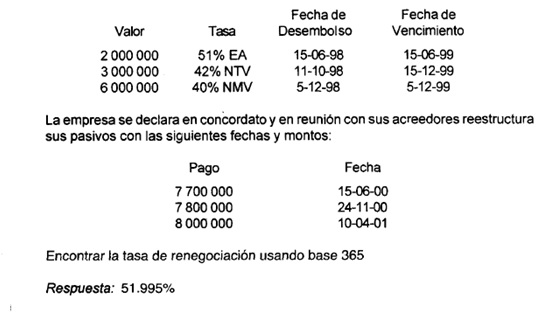
\includegraphics[height=9.2cm]{E2_33}
	\end{center}
	
\end{itemize}
\newpage


\chapter*{Capítulo 3}
\addcontentsline{toc}{chapter}{\textcolor{ocre}{Capítulo 3}}


\begin{itemize}
	
	\item 1. Se  constituye  un  CDT  a  180  días  por  \$650  000,  con  una  tasa  del  26\% naav  (nominal  anual  trimestre  vencido)  y  teniendo  en  cuenta  que  la retención en la fuente es del 7\%EA (anual efectiva) determinar:\\ 
	
	a. La tasa de interés(rentabilidad) antes de impuestos.\\
	b. La tasa de interés (rentabilidad) después de impuestos\\
	c. El valor en pesos que le entregan al vencimiento.\\
	d. Suponiendo una inflación del 18\% anual efectiva, determinar la tasa real obtenida.\\
	
	\textbf{Respuestas:} a.28,647\%  EA\hspace{0,5cm} b. 26,524\%  EA\hspace{0,5cm} c. \$731 139,01 d. 7.224\% EA\\
	\medskip
	
	\item 2. Un  inversionista  desea  obtener  una  rentabilidad  real  del  8\%  EA  (anual efectiva) ¿A qué tasa periódica debe invertir suponiendo que la inflación va a ser del 18\%EA?
	\medskip
	
	\textbf{Respuesta:} 27,44\% EA\\
	\medskip
	
	\item 3. Un  artículo  es  fabricado  en  Estados  Unidos  y  se  vende  en  Colombia  en \$50 000  ¿Cuánto  valdrá  el  artículo  en  Colombia  y  en  Estados  Unidos  al final  de  un  año,  suponiendo  los  siguientes  índices  económicos: cambio actual US\$1 = \$2 000, inflación en Estados Unidos 3\% EA, devaluación del peso 18\% EA?\\
	\textbf{Respuesta:} \$60 770 \hspace{0,5cm} US\$25,75\\
	\medskip
	\item 4. Un  artículo  es  fabricado en  Colombia  y  cuesta  \$68.000,  cuando  el cambio es de US\$1 = \$2 000. Suponiendo que el IPP de este sector en Colombia es del 22\% EA, y que la devaluación del peso frente al dólar sea del 18\%EA, hallar el precio del mismo artículo en cada país al final de un año.\\
	\medskip
	\textbf{Respuesta:} \$82 960 \hspace{0,5cm} US\$35,15\\
	\medskip
	\item 5. Dos  inversionistas  de  origen  alemán,  uno  residente  en  Alemania  y el  otro residente  en  Colombia,  han  decidido  realizar  un  negocio  en  Alemania  y cada uno aportará el 50\%. El negocio exige una inversión inicial de marcos  DM\$300 000   y   al   final   de   3   años   devolverá   la   suma   de   marcos DM\$400 000. Hallar las tasas totales y reales para cada uno de los socios suponiendo  que  los  siguientes  indicadores  económicos  se  mantuvieron estables durante los 3 años.\\
	
	a.tasa promedio de inflación en Colombia 22\% EA\\
	b.tasa promedio de inflación en Alemania 2\% EA\\
	c.   tasa  de  devaluación  del  peso  frente  al  dólar:  primer  año  18\% EA, segundo  año  20\% EA  y  tercer  año  17\% EA,  devaluación  marco frente  al  dólar:  años  1  y  2  el  2\% EA,  para  el  tercer  año  hay  una revaluación del 3\% EA\\
	d. cambio actual US\$ = DM\$2,23               US\$ = \$1 300\\
	\medskip
	\textbf{Respuestas:} En marcos 10.06\% EA y 7.9\% EA; en pesos: 29,85\% EA y 6,43\% EA.\\
	\medskip
	
	\item 6. El señor Yukimoto residente en el Japón y Mr.Jones residente en Estados Unidos  se  asocian para comprar un banco en Colombia, El valor de cada acción del banco es de \$9 000 pesos/acción y esperan venderla al final de 3 meses en \$9 700 pesos/acción. (Trabajar con 5 decimales).\\
	
	a. Cálcule la tasa de interés anual efectiva y la rentabilidad real(tasa de interés real) anual de cada uno de los socios\\
	b. ¿Cuánto tendrá cada uno en su respectiva moneda al final de los 3 meses?. Tome en cuenta la siguiente información:\\
	
	Inflación en: Colombia 18\% EA, en Estados Unidos 3.5\% EA, en Japón 2.3\%  EA tasa de devaluación del peso frente al dólar 22\%  EA tasa de devaluación del dólar frente al Yen 1\% EA Cambio actual US\$1 = \$2000; US\$1 = Yen105
	
	\textbf{Respuesta}:\\
	Yuquimoto i = 9.49465\% EA, $i_{R} = \$7 0347$\% EA\\
	Mr. Jones i = 10.60066\% EA, $i_{R} = \$6 86054$\% EA\\
	
	\medskip
	\item 7. Si en el problema anterior el valor del banco es de ochenta mil millones de pesos y Yukimoto  participa en el 40\% de la compra y Mr. Jones participa con el resto, determinar la cantidad que  recibirá c/u en su respectiva moneda.\\
	\textbf{Respuestas}:\\
	Yuquimoto Yenes 1.718.530.911.17\\ 
	Mr. Jones dólares US\$24.612 204.16\\
	
	\item 8. En el país A cuya moneda es el ABC, un par de zapatos vale 24 000 de ABC, existe una inflación  del 22\%EA y el cambio actual es de US\$1 =ABC 1 000. En el país X rige el dólar americano y se prevé  una inflación promedio del 6.5\% EA. Al final de un año ¿cuál debe ser la tasa de devaluación en A con respecto al dólar a fin de no perder competitividad en los mercados de X?\\
	\medskip
	\textbf{Respuesta:} 14.554\% EA
	\medskip
	\item 9. Un inversionista desea que todas sus inversiones le den una rentabilidad real del 5\% EA ¿Qué  tasa anual efectiva debe ofrecérsela si la inflación esperada es del 17\%EA de forma tal que satisfagan  los deseos del inversionista?
	
	\textbf{Respuesta:} 26.36\%EA\\ 
	\medskip
	\item 10. Un ahorrador consigna en una corporación de ahorro y vivienda la suma de \$300 000 el día 1 de  marzo y el día 20 de junio consigna \$200 000.  ¿Cuánto  podrá  retirar  el  31  de  agosto  si la corporación  paga el  27\% EA  (anual efectivo) de corrección monetaria para los meses de marzo y abril y el 25\% EA  para el resto del período (mayo, junio, julio y agosto).\\
	a. Elabore los cálculos en pesos\\
	b. Elabore los cálculos en UPAC sabiendo que el primero de marzo upac1 = \$6 650\\
	\textbf{Respuestas:} \$545 389 EA\hspace{0,5cm} UPAC 73.1415\\
	\medskip
	\item 11. Se estima que la corrección monetaria del primer año será del 18\% EA y la del segundo año del 17\% EA:\\
	a.Calcular la cantidad que antes de impuestos le entregarán a un inversionista que invierte la suma de \$800 000 a dos años en una cuenta de ahorros en UPAC que le garantiza pagar la corrección monetaria más el 4\% EA de interés sobre los UPAC.\\
	b. Calcule la rentabilidad (tasa de interés EA) obtenida antes de impúestos que el cambio actual es UPAC 1 = \$14000\\
	c. Si la retención en la fuente es del 7\% (anual efectiva) sobre los intereses, calcular la rentabilidad (tasa de interes EA) después de los impuestos\\
	d. Calcular la cantidad final que le entregarán después de impuestos\\
	\textbf{Respuestas:}a. \$1'194 605.57 \hspace{0,5cm} b. 22.199\% EA\hspace{0,5cm} c. 21,876\% EA\hspace{0,5cm} d. \$1'188 296.78\\
	\medskip
	\item 12. Hallar la tasa anual efectiva de;\\
	a. DTF +6 puntos\\
	b. IPC +7 puntos\\
	c Libor +8 puntos\\
	Asuma que: DTF = 15\% nata, IPC = 10\% nata, Libor = 5.14\% nasv (nominal semestre vencido)\\
	\textbf{Respuestas:} a.24.07\% EA\hspace{0,5cm} b.17.7\% EA\hspace{0,5cm} c.13.57\% EA\\
	\medskip
	\item 13. Suponiendo IPC = 8.5\% EA, CM= 12\% (CM= corrección monetaria), DTF = 15\% nata, TCC = 15.5\% nata, TBS (CF 180 días) = 19.27\% A.E., TBS(Bancos 360 días) = 19.19\% EA Hallar X de las siguientes igualdades:\\
	\textbf{Observación:} TBS (CF 180 días) significa tasa básica del sector corporaciones financieras a 180 días.\\
	
	a. IPC+10 = CM+x\\
	b. CM+14 = TCC+X\\
	c. DTF +8.6 = IPC+X\\
	d. TBS(CF 180 días) + 6 = DTF+x\\
	e. TCC+3.5 = DTF+X\\
	f. IPC+4 = DTF+X\\
	\textbf{Respuestas:}a.6.56\% EA\hspace{0,5cm} b.8.2\% nata EA\hspace{0,5cm} c.17.55\%A.E
	\\d.7.775\% nata\hspace{0,5cm} e.4\% nata\hspace{0,5cm} f. -3.1\% nata\\
	\medskip
	\item 14. Asumiendo que $i_{dev}$  = 25\%, IPC = 9\% EA, Prime Rate = 8.25\% EA, DTF = 14.5\% nata, Libor = 5\% EA, resolver las siguientes ecuaciones:\\
	
	$i_{DEV}$  + 10 = IPC +X\\
	$i_{DEV}$  +(Prime+ 200 p.b.) = DTF +X\\
	$i_{DEV}$  + (Libor + 500 p.b.) = DTF +X\\
	\textbf{Respuestas:} a. 26.148\% EA\hspace{0,5cm} EA. b. 16,32\% nata EA\hspace{0,5cm} c, 16,11\% nata\\
	\medskip
	\item 15. ¿Cuál es la rentabilidad efectiva anual del comprador (tasa de interés EA) y el precio de compra para el que adquiere una aceptación financiera a 180 días si se conserva hasta su maduración, se registra en bolsa a un precio de 86.225\% y la comisión de compra es del 0.5\% EA en rentabilidad?\\
	\textbf{Respuestas:} $i_{c} = 34\% EA\hspace{0,5cm}  P_{c} = 86,37\%$\\
	\medskip
	\item 16. ¿Cuál es la comisión en pesos para el problema anterior suponiendo que la aceptación financiera tiene un valor nominal de \$278 000?\\
	\textbf{Respuesta:} \$450\\
	\medskip
	\item 17. ¿Cuál es la rentabilidad efectiva anual que obtiene un inversionista que adquiere en el mercado secundario una aceptación bancaria emitida a 90 días con un precio de registro de 97.254\% y le faltan 28 días para su maduración? Suponga una comisión de compra del 0.4\% EA en rentabilidad. base 360.\\
	\textbf{Respuesta:} 42,645\% EA\\
	\medskip
	
	\item 18. Un exportador recibe una aceptación bancaria por sus mercancías la cual vence en 180 días, tiene una tasa de emisión del 28\% nasv  (Nominal anual semestre vencido). El mismo día en que le entregan la aceptación la ofrece en bolsa. Si las comisiones de compra y de venta son de 0,4\% EA y 0.6\% EA respectivamente, calcular:\\
	
	a.La tasa de registro\\
	b.La tasa del comprador\\
	c.La tasa del vendedor\\
	d.El precio de registro\\
	e.El precio de compra\\
	\textbf{Respuestas:} a. 29.36\% EA\hspace{0,5cm} b. 28.96\% EA\hspace{0,5cm}  c. 29.96\% EA\hspace{0,5cm} \\
	d. 87.922\% \hspace{0,5cm} e. 88.059\%.\\
	\medskip
	\item 19. Un inversionista compró el 14 de junio 98 una Aceptación Bancaria al 29.4\% EA con vencimiento el 15 de mayo/99 por \$250 millones, un segundo inversionista está dispuesto a adquirirlo el día 10 de septiembre/98 a una tasa del 34\% EA.\\
	
	a.¿Cuál será la utilidad en pesos del primer inversionista?\\
	b.¿Cuál es la rentabilidad del primer inversionista? (use un interés comercial es decir un año de 360 días).\\
	\textbf{Respuestas:} a. \$7 598 455\hspace{1.0cm} b. 17.14\% EA\\
	\medskip
	\item 20. Resuelva el problema anterior pero el segundo inversionista lo adquiere al 23.5\% EA\\
	\textbf{Respuestaa:} a. \$19 296 120\hspace{1,0cm} b. 47.8\% EA\\
	\medskip
	\item 21. Suponga que el señor X posee una aceptación financiera con valor de vencimiento de \$6 758 000 y desea venderla en Bolsa faltándole 57 días para vencerse y quiere ganarse un 29.5\% y la adquiere el señor Y. Suponga que la comisión de venta y de compra son 0.5\% EA y 0. 47\% EA respectivamente en rentabilidad. Base 365.\\
	
	a.¿Cuál es la tasa de registro?\\
	b.¿Cuál es el precio de registro?\\
	c. ¿Cuál la tasa que gana el señor Y?\\
	d.¿Cuál es el precio que paga el señor Y?\\
	e. ¿Cuál es la comisión de compra en pesos?\\
	\textbf{Respuestas:} a. $i_{R}= 29\%$EA\hspace{0,5cm} b. $P_{R} = \$6 494 534$\hspace{0,5cm}  c. $i_{c} = 28.53\%$ EA\hspace{0,5cm}\\
	d. Pc= \$6 498 237 \hspace{0,5cm} e. \$3 703\\
	\medskip
	\item 22. El señor XX posee una aceptación bancaria por valor de \$10 millones y la vende en Bolsa faltándole 87 días para su maduración, la adquiere el señor YY y el cual desea ganar el 32\% después de comisión pero antes de impuestos. Si la comisión de compra es del 0.4\% EA y la de venta el 0.375\% EA usando un año de 360 días determinar:\\
	
	a.	La tasa de registro\\
	b.	El precio de registro\\
	c.	La tasa de cesión\\
	d.	El precio de cesión\\
	e.	El precio al comprador\\
	f.	El valor en pesos de la retención en la fuente\\
	g.	La cantidad que debe pagar YY\\
	h.	La cantidad que recibe XX\\
	i.	La rentabilidad después de impuestos que gana YY\\
	\textbf{Respuestas:} a. $i_{R}$ = 32.4\% EA\hspace{0,5cm}  b. $P_{R}$ = \$9 344 234\hspace{0,5cm}   c. 32.775\% EA\hspace{0,5cm}  \\
	d. \$9 337 850\hspace{0,5cm}   e.  $P_{c}$ = \$9 351 070;  EA\hspace{0,5cm}    f. \$45 904;  \hspace{0,5cm}   g. \$9 396 974; \hspace{0,5cm}\\
	h. \$9 383 754 \hspace{0,5cm} EA\hspace{0,5cm}   i. 29.352\% EA.\\
	\medskip
	\item 23. En el problema 21 calcule el valor que recibe el vendedor y el valor que paga el comprador suponiendo que la retención en la fuente es del 7\% EA sobre utilidades.\\
	\textbf{Respuestas:}\\
	El comprador paga \$6 516 680,\\
	Vendedor recibe \$6 509 055.\\
	\medskip
	\item 24. El 27 de abril de 1999 se compra una aceptación bancaria de \$36 millones en el mercado bursátil, con vencimiento el 27 de julio de 1999 y con tasa de registro del 26\% EA (anual efectiva). Si después de transcurridos 34 días la vende. ¿Qué precio se debe cobrar si el vendedor desea obtener una rentabilidad durante la tenencia del 26.5\% EA?\\
	Base 365.\\
	\textbf{Respuesta}: $P_{v}$ = \$34 736 688\\
	\medskip
	\item 25. Resuelva el problema anterior suponiendo que el corredor cobra una comisión del 0.1\% en rentabilidad y que de todas maneras el vendedor quiere ganarse el 26.6\% EA durante la tenencia.\\
	\textbf{Respuesta:} $P_{v}$ =\$34 746 123\\
	
	
\end{itemize}

%%%%%%%%%%%%%%%%%%%%%%%%%%%%%%%%%%%%%%%%%%%%%%%%%%%%%%%%%%%%%%%%%%%%%%%%%%%%%%%


\chapter*{Capítulo 4}
\addcontentsline{toc}{chapter}{\textcolor{ocre}{Capítulo 4}}


\begin{itemize}
	
	\item 1. Hallar el monto y el valor presente de 20 pagos de \$2000 c/u, suponga una tasa del 18\% EA.\\
	\textbf{Respuesta:} Monto: \$293.255,94 \hspace{1,5cm} Valor Presente: \$10.705,49\\
	\medskip
	\item 2. Para la compra de un automóvil que vale \$6 000 000; se exige una cuota inicial del 40\% y el resto se cancela en 36 cuotas mensuales, ¿a cuánto ascenderá la cuota, si los intereses son del 3.5\% pmv\\
	\textbf{Respuesta:} \$177.422,99\\
	\medskip
	\item 3. Si en el problema anterior se ofrecen 2 cuotas extraordinarias: la primera de
	\$350.000 en el mes 5, y la segunda de \$500.000, en el mes 18, ¿cuál será el valor de la cuota ordinaria?\\
	\textbf{Respuesta:} \$149.633,07\\
	\medskip
	\item 4. Una persona va a comprar una máquina que vale \$800.000, con el objeto de poder disponer de esa cantidad el 15 de diciembre de 1989. Comienza a hacer depósitos mensuales de \$R, en un fondo que paga el 30\% namv. Si el primer depósito lo hace el 15 de febrero de 1988, Hallar el valor del depósito mensual.\\
	\textbf{Respuesta:} \$26.157,10\\
	\medskip
	\item 5. Un documento estipula pagos trimestrales de \$10.000 iniciando el primer pago el 20 de enero de 1987 y terminando el 20 de julio de 1995: Si se desea cambiar este documento por otro que estipule pagos trimestrales de \$R, comenzando el 20 de abril de 1988 y terminando el 20 de julio de 1989, Hallar el valor de la cuota. Suponga una tasa del 20\% natv. \textbf{Sugerencia}: El valor de los documentos debe ser igual en el punto que escoja como fecha focal.\\
	\textbf{Respuesta:} \$41.172,87\\
	\medskip
	\item 6. Una persona se compromete a pagar \$60.000 mensuales, a partir del 8 de julio de 1988 hasta el 8 de diciembre de 1989. Para dar cumplimiento a ese contrato, se propone hacer depósitos mensuales de \$R c/u, en una cuenta de ahorros que como mínimo le garantiza el 1.5\% pmv (periódico mes vencido). Si el primer depósito lo efectúa el 8 de marzo de 1986, ¿cuál será el valor de \$R (valor de la serie uniforme), suponiendo que el último depósito lo hará:\\
	
	a, El 8 de diciembre de 1989\\
	b. El 8 de julio de 1988\\
	c. El 8 de junio de 1988\\
	d. El 8 de abril de 1987\\
	\textbf{Respuestas:} a. \$18.749\hspace{1,5cm} b. \$26.514\hspace{1,5cm} c. \$27.271\hspace{1,5cm} d. \$49.411\\
	\medskip
	\item 7. Una deuda de \$800.000 va a ser cancelado en pagos trimestrales de \$78.000 durante tanto tiempo como fuere necesario. Suponiendo una tasa del 30\% natv.\\
	
	a. ¿Cuántos pagos de \$78.000 deben hacerse?\\
	b. ¿Con qué pago final hecho 3 meses después del último pago de \$78.000 cancelará la deuda?\\
	\textbf{Respuesta:} a. 20\hspace{1,5cm} b. \$22.054,42\\
	\medskip
	\item 8. Resuelva el problema anterior si la tasa es del 42\% natv. Justifique su respuesta desde el punto de vista matemático y desde el punto de vista financiero.\\
	\textbf{Respuesta:} No hay solución\\
	\medskip
	\item 9. Desean reunirse exactamente \$60.000 mediante depósitos mensuales de \$1.000, en un fondo que paga el 36\% namv.\\
	
	a. ¿Cuántos depósitos de \$1.000 deberán hacerse?\\
	b. ¿Qué depósito adicional hecho conjuntamente con el último depósito de \$1.000 completará los \$60.000?\\
	c. ¿Qué depósito adicional hecho un mes después del último depósito de \$1.000 completará los \$60.000?\\
	\textbf{Respuestas:} a. 34 pagos  \hspace{1,5cm} b. \$2.270\hspace{1,5cm}  c. \$538\\
	\medskip
	\item 10. Resolver el problema anterior incluyendo un depósito adicional de \$7.000 en el período 10.\\
	\textbf{Respuesta:} a. 29 pagos\hspace{1,5cm} b. \$2.507\hspace{1,5cm} c.\$782\\
	\medskip
	\item 11. Para cancelar una deuda de \$80.000, con intereses al 24\% namv se hacen pagos mensuales de \$3.000 cada uno.\\
	
	a.¿Cuántos pagos de \$3.000 deben hacerse?\\
	b.¿Con qué pago adicional hecho conjuntamente con el último pago de \$3.000 se cancelará la deuda?\\
	c. ¿Qué pago adicional hecho un mes después del último pago de \$3.000 cancelará la deuda?\\
	\textbf{Respuesta:} a. 38 pagos\hspace{1,5cm} b. \$1.439\hspace{1,5cm} e. \$1.468\\
	\medskip
	\item 12. Resolver el problema anterior suponiendo que se hace un pago adicional de \$10.000 con la décima cuota.\\
	\textbf{Respuesta:}a. 32 pagos \hspace{1,5cm} b. \$2.622 \hspace{1,5cm} c. \$2.675\\
	\medskip
	\item 13. Una máquina cuesta al contado \$600.000, para promover las ventas, se ofrece que puede ser vendida en 24 cuotas mensuales iguales, efectuándose la primera el día de la venta. Si se carga un interés del 3\% pmv (periódico mes vencido). Calcular el valor de cada pago.\\
	\textbf{Respuesta:} \$34.396,55\\
	\medskip
	\item 14. Un fondo para empleados presta a un socio la suma de \$2 millones para ser pagado en 3 años, mediante cuotas mensuales uniformes, con intereses sobre saldos al 24\% namv. Si en el momento de pagar la sexta cuota, decide pagar en forma anticipada las cuotas 7, 8 y 9:\\
	
	a. ¿cuál debe ser el valor a cancelar al vencimiento de la sexta cuota?\\
	b. ¿cuál debe ser el valor de los intereses descontados?\\
	\textbf{Respuestas:} a. \$304.751,66 \hspace{1,5cm}b. \$9.111\\
	\medskip
	\item 15. Una  persona adopta un plan de ahorros del fondo ABC, que establece depósitos mensuales de \$1.000, comenzando el primero de febrero de 1986 hasta el primero de abril de 1987 y, depósitos mensuales de \$2.000, desde el primero de mayo de 1987 hasta el primero de diciembre de 1987. El capital así reunido permanecerá en el fondo hasta el primero de junio de 1988, fecha en la cual le será entregado al suscriptor junto con intereses calculados al 12\% namv. \\
	
	El plan anterior estaba funcionando perfectamente según lo proyectado pero, por razones comerciales la junta directiva del fondo ABC decidió que, a partir del primero de octubre de 1986, el fondo pagará a todos sus clientes de ahorros el 18\% namv. ¿Cuál será el capital que, el primero de junio de 1988, le entregarán a la persona que ha decidido adoptar el plan?\\
	
	\textbf{Respuesta:} \$38.733\\
	\medskip
	\item 16. Un contrato de arriendo por un año establece el pago de \$20.000 mensuales al principio de cada mes. Si ofrecen cancelar todo el contrato a su inicio, ¿cuánto deberá pagar?. Suponiendo:\\
	
	a. tasa del 30\% nama (Nominal Anual mes anticipado).\\
	b. tasa 3\% pma (periódica mes anticipado)\\
	\textbf{Respuestas:} a.\$210.284 \hspace{1,5 cm} b. \$204.105\\
	\medskip
	\item 17. Una máquina produce 2.000 unidades mensuales las cuales deben venderse a \$80 c/u. El estado actual de la máquina es regular y si no se repara podría servir durante 6 meses más y luego desecharla, pero si hoy le hacemos una reparación total a un costo de \$800.000, se garantizaría que la máquina podría servir durante un año contado a partir de su reparación. Suponiendo una tasa del 4\% pma ¿será aconsejable repararla?\\
	\textbf{Respuesta:} No es aconsejable repararla\\
	\medskip
	\item 18. Elaborar una tabla para amortizar la suma de \$3 millones en pagos trimestrales durante 15 meses con una tasa del 46\% natv.\\
	\textbf{Respuesta parcial:} Cuota \$821.945,32 Trimestral\\
	\medskip
	\item 19. Elaborar una tabla para capitalizar la suma de \$2 millones mediante depósitos semestrales durante 3 años. Suponga una tasa del 42\% nasv\\
	\textbf{Respuesta parcial:} Depósito \$196.405,92 Semestral\\
	\medskip
	\item 20. Una persona desea reunir \$800.000 mediante depósitos mensuales de \$R c/u durante 5 años en una cuenta que paga el 30\% namv. ¿Cuál es el total de intereses ganados hasta el mes 30?\\
	\textbf{Respuesta:} \$81.785,81\\
	\medskip
	\item 21. Para cancelar una deuda de \$2 millones con intereses al 36\% namv se hacen pagos mensuales de \$R c/u, durante 15 años.\\
	
	a. Calcular el valor de la deuda después de haber hecho el pago número 110\\
	b. Calcular el total de los intereses pagados hasta el mes 110\\
	\textbf{Sugerencia:}para la parte a. calcule el valor presente en el mes 110  de los 70 pagos que falta por cancelar, para la parte b. halle la diferencia entre el total pagado y el total amortizado.
	\textbf{Respuestas:} a. \$1'755.991,89 \hspace{1,5 cm} b. \$6'388.423,79\\
	\medskip
	\item 22. Se necesita \$1 millón, para realizar un proyecto de ampliación de una bodega, una compañía A ofrece prestar el dinero, pero exige que le sea pagado en 60 cuotas mensuales vencidas de \$36.132,96 c/u. La compañía B ofrece prestar el dinero, pero para que le sea pagado en 60 pagos mensuales de \$19.000 c/u y dos cuotas adicionales así: la primera de \$250.000, pagadera al final del mes 12, la segunda, de \$350.000, pagadera al final del mes 24. Hallar la tasa periódica mensual vencida que cobra cada uno, para decidir que préstamo debe utilizar.\\
	\textbf{Respuesta:} A. 3\% pmv (periódico mes vencido) \hspace{0,5 cm}              B. 2,35\% pmv\\
	Utilice la compañía B.\\
	\medskip
	\item 23. Un equipo de sonido cuesta \$400.000 al contado, pero puede ser cancelado en 24 cuotas mensuales de \$33.000 c/u efectuándose la primera el día de la venta. ¿Qué tasa pma (periódica mes anticipada) se está cobrando?\\
	\textbf{Repuesta:} 7,159\% pma\\
	\medskip
	\item 24. ¿A qué tasa nominal, namv (Nominal anual  mes vencido), está siendo amortizada una deuda de \$300.000, mediante pagos mensuales de \$10.000, durante 4 años?\\
	\textbf{Respuesta:} 25,32\% namv (Nominal anual mes vencido)\\
	\medskip
	\item 25. ¿A qué tasa nominal, naav (Nominal anual trimestre vencido), está reuniéndose un capital de \$400.000 mediante depósitos trimestrales de \$20.000 c/u durante 3 años?\\
	\textbf{Respuesta:} 35,53\% naav\\
	\medskip
	\item 26. Una entidad financiera me propone que le deposite mensualmente \$10.000 durante 3 años comenzando el primer depósito el día de hoy y me promete devolver al final de este tiempo la suma de \$7'000.000. ¿Qué tasa pma me va a pagar?\\
	\textbf{Respuesta:} 13\% pma\\
	\medskip
	\item 27. Un señor compró un automóvil, dando una cuota inicial del 20\% y el saldo lo cancela con cuotas mensuales de \$317.689,78 durante 3 años. Después de efectuar el pago de la cuota 24 ofrece cancelar el saldo de la deuda de un solo contado y le dicen que su saldo en ese momento asciende a la suma de \$3'060.928,56.\\
	
	a. Calcular con 2 decimales exactos la tasa (periódica mes vencido) que le están cobrando.\\
	b. Calcular la tasa efectiva anual EA equivalente que le cobran.\\
	c. ¿Cuál es el costo total del automóvil?\\
	\textbf{Respuestas:} a. 3.55\% pmv  \hspace{0,5cm} b. 52\% EA  \hspace{0,5cm} c.\$8 millones
	
\end{itemize}\
\newpage

%%%%%%%%%%%%%%%%%%%%%%%%%%%%%%%%%%%%%%%%%%%%%%%%%%%%%%%%%%%%%%%%%%%%%%%%%%%%%%%%

\chapter*{Capítulo 5}
\addcontentsline{toc}{chapter}{\textcolor{ocre}{Capítulo 5}}



\begin{itemize}
	
	\item 1. Cuando su hijo cumple 12 años, un padre hace un depósito de \$X en una fiduciaria, con el objeto de asegurar sus estudios universitarios, los cuales iniciará cuando cumpla 20 años. Suponiendo que para esa época el valor de la matrícula anual en la universidad será de \$300.000 y que permanecerá constante durante los seis años que duran los estudios universitarios, ¿cuál debe ser el valor de \$X? Suponga una tasa del 30\% EA, anual efectiva.\\
	\textbf{Respuesta:} \$126.349.41\\
	\medskip
	
	\item 2. Una persona necesita comprar hoy una máquina, el modelo A cuesta \$300.000; el modelo B, \$500.000, el C \$700.000 y el modelo D, \$900.000. Si la persona puede hacer 36 pagos mensuales de máximo \$30.000 durante 3 años, pero comenzando el primer pago al final de 6 meses ¿cuál será el modelo más costoso que podrá comprar? Suponga una tasa del 30\% namv (Nominal anual mes vencido).\\
	\textbf{Respuesta:} El valor presente de lo que puede pagar es \$624.608.81 por tanto decida modelo B.\\
	\medskip
	
	\item 3. Una persona solicita un préstamo el día 1 de marzo de 1989 y planea efectuar pagos mensuales de \$12.000, desde el 1 de octubre de 1989, hasta el 1 de agosto de 1990. Si le cobran un interés del 3.5\% pmv (periódico mes vencido), ¿cuál será el valor del préstamo?\\
	\textbf{Respuesta: \$87.873.21}\\
	\medskip
	
	\item 4. Un filantrópico ha creado una institución de caridad y desea asegurar su funcionamiento a perpetuidad. Se estima que esta institución necesita para su funcionamiento \$100.000, al final de cada mes, durante el primer año; \$200.000, al final de cada mes, durante el segundo año y \$300.000, al final de cada mes, en forma indefinida. Suponiendo una tasa del 30\% namv (Nominal anual mes vencido), hallar el valor de la dote (Se denomina dote al valor único que, entregado al principio, asegura el mantenimiento a perpetuidad, en el caso de las personas el mantenimiento es vitalicio).\\
	\textbf{Respuesta:} \$9.185.725\\
	\medskip
	
	\item 5. Un señor deposita el primero de abril de 1986 \$10.000, en un fondo que paga el 36\% namv (Nominal anual Semestre vencido).\\
	
	a. ¿cuántos retiros semestrales de \$8.000 podrá hacer, si el primer retiro lo hace el primero de abril de 1989?\\
	b. ¿cuál será el valor del retiro adicional que hecho un período después del último pago de \$8.000 cancelará el fondo?\\
	\textbf{Respuestas:} a. 4 períodos \hspace{1,0cm} b. \$3104,68\\
	\medskip
	
	\item 6. Suponiendo una tasa del 36\% namv (Nominal anual mes vencido), ¿cuál será el valor presente de:\\
	
	a.\$200.000, al final de cada mes, en forma indefinida\\
	b.\$200.000, al principio de cada mes indefinidamente?\\
	\textbf{Respuestas:} a. \$6.666.666.67 \hspace{0,5 cm}b, \$6.866.666.67 con tasa del 36\% nama (Nominal anual mes anticipada\\
	\medskip
	
	\item 7. Un inversionista deposita hoy \$100.000 y \$300.000, en 3 años; al final del año 5, comienza a hacer depósitos anuales de \$50.000, durante 6 años, ¿cuánto dinero podrá retirarse en forma indefinida, comenzado al final del año 14? Utilice una tasa del 20\% EA (anual efectiva).\\
	\textbf{Respuesta:} \$757.080\\
	\medskip
	
	\item 8. Un grupo de benefactores decide dotar a un hospital de los equipos de laboratorio que necesita, se estima que el costo de los equipos el día primero de julio de 1990 será de \$4 millones y que necesitará \$300.000 trimestralmente, como costo de funcionamiento en forma indefinida, a partir del primero de abril de 1991, fecha en la cual entrará en funcionamiento. ¿Cuál debe ser el valor de la donación que se haga el día primero de enero de 1990 si el dinero es invertido inmediatamente en una fiduciaria que garantiza el 24\%  naav (Nominal anual Trimestre vencido)?\\
	\textbf{Respuesta:} \$7'520.454.\\
	\medskip
	
	\item 9 Una empresa pretende tomar una casa-lote que requiere la suma de \$2.000.000 anuales como costo de mantenimiento y de \$3.000.000 cada 4 años para reparaciones adicionales. Por otra casa-lote que le ofrecen, se requerirá de una suma de \$3.000.000 anuales para mantenimiento y de \$2.500.000 cada tres años para reparaciones adicionales. Si la casa-lote se usará por tiempo indefinido y suponiendo una tasa de interés del 35\% EA (anual efectiva), ¿cuál de las dos alternativas es más conveniente tomar?\\
	\textbf{Respuesta:} Primera alternativa \$7.006.550; segunda alternativa \$10.283.318. Decidir primera alternativa.\\
	\medskip
	
	\item 10. Con interés al 24\%  naav (Nominal anual Trimestre vencido), ¿cuál debe ser valor de los pagos semestrales vencidos que, hechos por 10 años, amortizarán una deuda de \$1.200.000?\\
	\textbf{Respuesta:} \$164.293
	\medskip
	
	\item 11. Resolver el problema anterior si los pagos son anticipados.\\
	\textbf{Respuesta:} \$146.220\\
	\medskip
	
	\item 12. Una persona compra un artículo por \$600.000. Sí da una cuota inicial del 40\% y cancela el saldo, en cuotas trimestrales vencidas, de \$50.000, cancelará la deuda.\\
	\textbf{Respuesta:} 12 pagos de \$50.000, y un pago final de \$21.631.\\
	\medskip
	
	\item 13. Si se deposita mensualmente la suma de \$1.000 en un fondo que paga el 27\%  namv (Nominal anual Mes vencido) y adicionalmente, deposita de \$.2000 cada 3 meses ¿Cuánto se habrá acumulado, al final de 5 años?
	\textbf{Respuesta:} \$205.578
	\medskip
	
	\item 14. Con  el objeto de poder hacer 10 retiros semestrales de \$70.000, se depositan hoy un capital en una cuenta de ahorros que paga el 21\%  naav (Nominal anual Trimestre vencido). Si el primer retiro lo hace al final de un año, ¿cuál debe ser el valor de la cuenta?
	\textbf{Respuesta:} \$375.673\\
	\medskip
	
	\item 15. Un señor desea comprar una póliza de seguro que garantice a su esposa el pago de \$40.000 mensuales durante 10 años y adicionalmente \$50.000 al final de cada año durante este mismo período. Si el primer pago se efectúa al mes del fallecimiento del señor, hallar el valor de la póliza de seguro suponiendo que la compañía de seguros garantiza el 24\%  naav (Nominal anual Trimestre Vencido).\\
	\textbf{Respuesta:} \$1'983 299.51\\
	\medskip
	
	\item 16. Se desea cancelar una deuda de \$900.000 en pagos mensuales de \$R durante 3 años, el primero al final de un mes, y además se efectuaran abonos semestrales extraordinarios de una y media veces la cuota ordinaria, el primero de estos al final de 6 meses. Suponiendo una tasa del 36\% namv. ¿Cuál debe ser el valor de las cuotas ordinarias y el de las cuotas extraordinarias?\\
	\textbf{Respuesta:} a.\$33.463.38 \hspace{0,5cm} b. \$50.195.07\\
	\medskip
	
	\item 17. Se compra un carro en \$12.000.000 mediante el pago de 48 cuotas mensuales vencidas de \$R c/u y cuotas trimestrales vencidas de \$400.000 c/u durante 4 años. Si se cobra una tasa del 44\% EA  anual efectivo, determinar el valor de \$R.\\
	\textbf{Respuesta:} \$353.137.09\\
	\medskip
	
	\item 18. Con una tasa del 25\% EA  anual efectivo, ¿cuál debe ser el valor presente de una serie uniforme infinita de \$600.000 al final de cada 4 años? Utilice cambio de tasa.\\
	\textbf{Respuesta:} \$416.260\\
	\medskip
	
	\item 19. Resuelva el problema anterior modificando los pagos\\
	\textbf{Respuesta:} \$416.260\\
	\medskip
	
	\item 20. Reemplazar pagos de \$200.000 hechos cada 2 años por pagos equivalentes cada 5 años suponiendo una tasa del 30\% EA\\
	\textbf{Respuesta:} \$786.356.52 cada 5 años.
	\medskip
	
	\item 21. Con una tasa del 20\% EA anual efectivo, ¿qué es más conveniente para una universidad, recibir una renta perpetua de \$800.000 cada 5 años comenzando el primer pago en el cuarto año, 0 recibir \$200.000 anuales de renta perpetua comenzando el primero dentro de un año?\\
	\textbf{Respuesta:} La primera opción le representa \$ 645.022.58 pesos de hoy y la segunda opción le representa \$1 millón en pesos de hoy, por tanto, es mejor la segunda opción.\\
	\medskip
	
	\item 22. Una máquina llegará al final de su vida útil dentro de 2 años, para esa época una nueva máquina que se adquiera costará \$900.000 y se estima que la máquina vieja podrá ser recibida en parte de pago de la nueva en la suma de \$200.000. ¿Qué depósito trimestral debo hacer en una cuenta que paga el 30\% namv, con el objeto de hacer la compra en el momento oportuno si el primer depósito lo hago al final de 6 meses?\\
	\textbf{Respuesta:} \$79.200.82\\
	\medskip
	
	\item 23. Una fábrica se puede comprar en la suma de \$1 millón, la cual produce 2.000 unidades mensuales de un cierto artículo que podrá ser vendido durante los primeros 6 meses a \$30 la unidad y en \$50 la unidad durante los siguientes 6 meses. El inversionista piensa que podrá vender la fábrica al final de un año en la suma de \$1.2 millones. Si el inversionista gana normalmente en todos sus negocios el 5\% pmv (periódico mensual vencido), le aconsejaría usted que comprara la fábrica?\\
	\textbf{Respuesta:} Si porque en pesos de hoy los ingresos suman \$1.351.502.38 y los egresos son \$1 millón\\
	\medskip
	
	\item 24. Calcular la tasa que gana el inversionista del problema anterior.\\
	\textbf{Respuesta}: 8.54\% pmv (periódico mensual vencido).\\
	\medskip
	
	\item 25. Hoy primero de noviembre de 1999 se tiene una obligación a la que le restan 18 cuotas mensuales anticipadas de \$827.643 c/u para terminar de pagarse. El acreedor desea cambiar la forma de pago de su deuda y pacta realizar 10 pagos trimestrales vencidos de \$2.965.345.96 c/u. ¿En qué fecha deberá realizar el primer pago de la nueva anualidad? Utilice una tasa del 38.5\% efectivo anual.\\
	\textbf{Respuesta:} Primero de agosto del año 2001\\
	\medskip
	
	\item 26. Se concede un préstamo de \$20 millones para ser pagado en cuotas mensuales en la siguientes condiciones:\\
	
	a. En los primeros 6 meses no se efectuara ningún pago pero los intereses si se causan (esto es un período de gracia)\\
	b. En los siguientes 6 meses se pagará la suma de \$600.000 mensualmente\\
	c. De el mes 13 en adelante se pagará mensualmente la suma de \$R\\
	d. Plazo total 3 años. (En este tiempo queda incluido el período de gracia)\\
	e. Durante el primer año se cobrará un interés del 12\% namv, durante el segundo año se cobrara una tasa del 18\%  namv, y durante el tercer año se cobrará una tasa del 24\%  namv.\\
	Determinar el valor de \$R\\
	\textbf{Respuesta:} \$954.066.98\\
	\medskip
	
	\item 27. Por un préstamo de 15 millones se exige el pago de \$450.000 mensuales durante los primeros 12 meses, de \$600.000 por los siguientes 12 meses, de \$1 millón mensual por los siguientes 12 meses y un pago final de \$2 millones en el mes 3. ¿Cuál es la tasa de interés periódica mensual que se está cobrando?\\
	\textbf{Respuesta:} 2.725\% periódico mensual vencido.\\
	
	\item 28. Resolver el problema anterior suponiendo que a partir del segundo año se cobra una tasa de interés igual al doble de la que se cobra en el primer año.\\ 
	\textbf{Sugerencia:} Resuelva el problema por Excel.\\
	\textbf{Respuesta:} tasa del primer año 1.4356\% periódico mensual vencido y de ahí en adelante el 2.8712\% periódico mensual vencido.\\
	
\end{itemize}
\newpage
%%%%%%%%%%%%%%%%%%%%%%%%%%%%%%%%%%%%%%%%%%%%%%%%%%%%%%%%%%%%%%%%%%%%%%%%%%%%%%%%%

\chapter*{Capítulo 6}
\addcontentsline{toc}{chapter}{\textcolor{ocre}{Capítulo 6}}


\begin{itemize}
	\item 1. Un documento exige hacer 12 pagos mensuales vencidos. Si el primer pago es de \$6 000 y c/u disminuye en \$800.\\
	
	a. ¿Cuál será el valor del último pago?\\
	b. ¿Cuál será el valor final de todos ellos, suponiendo una tasa del 36\% namv?\\
	\textbf{Respuestas:} a. \$2 800 \hspace{ 0,5cm} b. \$26698.06\\
	\medskip
	
	\item 2. Hallar el valor presente de 15 pagos que decrecen linealmente en \$400, si el primer pago es de \$5 000 y la tasa efectiva es del 4\% EA\\.
	\textbf{Respuesta:} \$27 697.74\\
	\medskip
	
	\item 3. Con interés efectivo del 10\% EA, hallar el valor final del siguiente flujo de caja:\\
	\begin{center}
		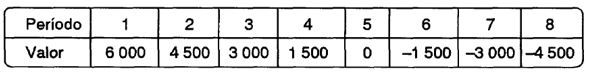
\includegraphics[height = 2.0cm]{E6_3}
	\end{center}
	\textbf{Respuesta:} \$17077\\
	\medskip
	
	\item 4. Hallar el valor de \$R del siguiente flujo de caja, con intereses al 30\% EA\\.
	\begin{center}
		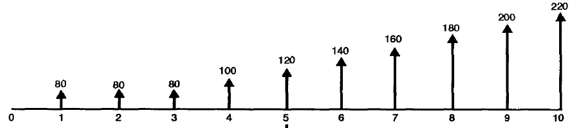
\includegraphics[height = 3.0cm]{E6_4}
	\end{center}
	\textbf{Respuesta:} \$1 203,02\\
	\medskip
	
	\item 5. Hallar \$R del siguiente flujo de caja, con tasa del 20\% EA.    
	\begin{center}
		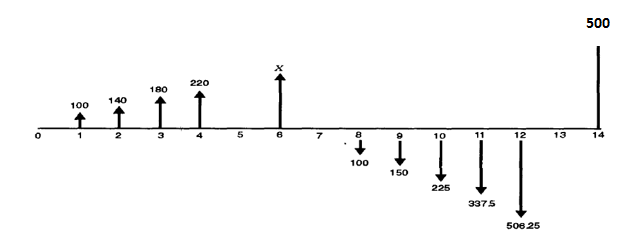
\includegraphics[height = 5.5cm]{E6_5}
	\end{center}
	\textbf{Respuesta:} \$713.33. Significa que R tiene sentido opuesto al que aparece en la gráfica.\\
	\medskip
	
	\item 6. Con tasa del 25\% EA, hallar \$R del siguiente flujo de caja.
	\begin{center}
		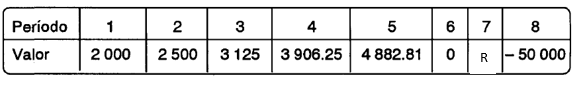
\includegraphics[height = 2.0cm]{E6_6}
	\end{center}
	\textbf{Respuesta:} \$1 853.03\\
	\medskip
	
	\item 7. Hallar el primer pago de un gradiente lineal creciente en \$300, que tenga 50 pagos anuales y que sea equivalente a 50 pagos anuales que crecen un 20\%, con primer pago de \$1 000, suponga una tasa del 20\% EA\\.
	\textbf{Respuesta:} \$6 835.90\\
	\medskip
	
	\item 8. Una persona quiere comprar un automóvil, que actualmente cuesta \$4 millones; para tal fin, decide establecer un fondo mediante depósitos mensuales crecientes en un 4\%. Si el primer depósito es de \$60000, que se hace al final de un mes, ¿cuánto tiempo le llevará reunir el dinero necesario para la compra, si el automóvil sube de precio cada mes un 1\%? Suponga una tasa del 4\% periódico mensual vencido.\\
	\textbf{Sugerencia:} Calcule el tiempo por interpolación.\\
	\textbf{Respuesta:} 29.35 meses, luego debe esperar 30 meses.\\
	\medskip
	
	\item 9. ¿Cuántos pagos mensuales deben hacerse para cancelar una deuda de \$2 millones, con intereses del 36\% namv, suponga que la primera cuota es de \$50000 y que la cuota crece en \$500 mensualmente.\\
	\textbf{Respuesta:} Por interpolación 96.29 períodos, luego debe esperar 97 períodos.\\
	\medskip
	
	\item 10. Con interés efectivo del 14\%, hallar el valor final de la siguiente serie:\\
	\begin{center}
		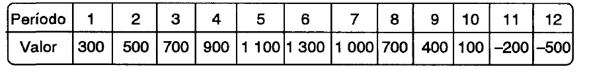
\includegraphics[height = 2.0cm]{E6_10}
	\end{center}
	\textbf{Respuesta:} \$16673.39\\
	\medskip
	
	\item 11. Con interés efectivo del 10\% EA hallar el valor presente de la siguiente serie utilizando gradientes: 
	\begin{center}
		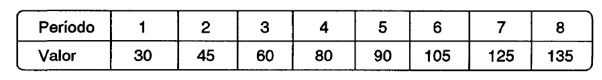
\includegraphics[height = 2.0cm]{E6_11}
	\end{center}
	\textbf{Sugerencia:} divida las cuotas de los períodos 4 y 7, de forma tal que una parte esté de acuerdo con la ley de formación del gradiente y el excedente lo puede considerar como cuota adicional.\\
	\textbf{Respuesta:} \$406.46\
	\medskip
	
	\item 12. Con interés efectivo del 10\%, hallar el valor presente de la siguiente serie utilizando gradientes:\\
	\begin{center}
		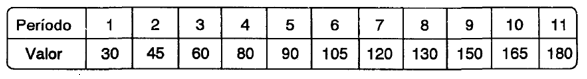
\includegraphics[height = 2.0cm]{E6_12}
	\end{center}
	\textbf{Respuesta:} \$591.87\\
	\medskip
	
	\item 13. Con una tasa del 6\% EA hallar el valor presente de la siguiente serie usando gradiente.\\
	\begin{center}
		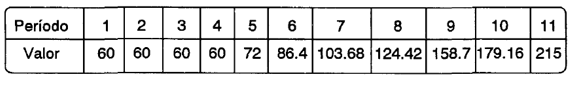
\includegraphics[height = 2.0cm]{E6_13}
	\end{center}
	\textbf{Respuesta:} \$776.86\\
	\medskip
	
	\item 14. Hallar el valor presente de una serie infinita de pagos si el primero vale \$1 000 y son crecientes en un 10\%. Suponga una tasa efectiva del 8\%\\.
	\textbf{Respuesta:} Infinito\\
	\medskip
	
	\item 15. ¿Cuál es el valor presente de una serie infinita de pagos mensuales que crecen cada mes en \$3000 y cuyo primer pago es de \$20 000. Suponga una tasa del 2.5\% pmv.\\
	\textbf{Respuesta:} \$5'600 000\\
	\medskip
	
	\item 16. Para mantener en buen estado una carretera veredal, los hacendados de la región desean establecer un fondo, para proveer las reparaciones futuras. Estas se estiman en un millón de pesos para el próximo año; también, se estima que su costo se incrementará todos los años en un 18\%. Hallar el valor del fondo, suponiendo un interés del 28\% EA\\.
	\textbf{Respuesta:} \$10.000 000\\
	\medskip
	
	\item 17.Hallar el valor presente de 24 pagos mensuales que crecen cada mes un 2\%. Suponga una tasa del 2\% pmv y que el primer pago es de \$5 000.\\
	\textbf{Respuesta:} \$117 647.06\\
	\medskip
	
	\item 18.Hallar el valor presente de un gradiente infinito de pagos mensuales que crecen un 2\% y cuyo primer pago es de \$8 000\\.
	
	a. Suponga una tasa del 3\% pmv.\\
	b Suponga una tasa del 1,5\% pmv.\\
	\textbf{Respuesta:} a \$800 000 \hspace{0,5 cm}  b. Infinito\\
	
	\item 19.¿A qué tasa anual efectiva se cumplen las condiciones mostradas en el siguiente diagrama?\\
	\begin{center}
		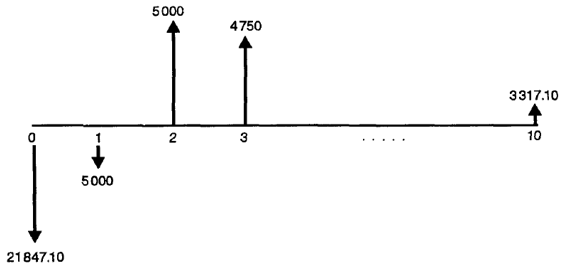
\includegraphics[height = 5.0cm]{E6_19}
	\end{center}
	\textbf{Respuesta:} 6.25\% EA\\
	\medskip
	
	\item 20. ¿A qué tasa efectiva se cumplen las condiciones mostradas en el siguiente diagrama?\\
	\begin{center}
		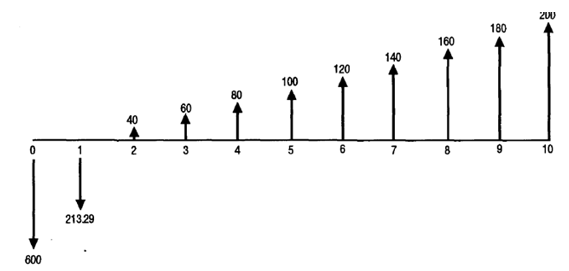
\includegraphics[height = 5.3cm]{E6_20}
	\end{center}
	\textbf{Respuesta:} 4,3\% EA\\
	\medskip
	
	\item 21. Reemplazar el siguiente flujo de caja, por una serie uniforme, de igual número de pagos anuales, con una tasa del 20\% EA.\\
	\begin{center}
		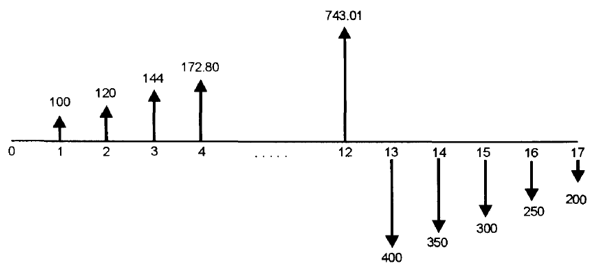
\includegraphics[height = 5.3cm]{E6_21}
	\end{center}
	\textbf{Respuesta:} 187,10\%\\
	\medskip
	
	\item 22. Un padre desea reunir una cantidad mediante depósitos anuales uniformes, comenzando hoy (primero de enero de 1984) y terminando el primero de enero de 1990, en un fondo que paga el 28\% nasv, su objetivo es el de garantizar a su hijo el estudio universitario, que se estima durará unos 6 años y empezará el primero de enero de 1990. Actualmente, la matrícula semestral cuesta \$30.000, pero aumentará todos los semestres un 8\%. Calcular el valor de los depósitos anuales.\\ 
	\textbf{Sugerencia:} calcular el valor de la matrícula el primero de enero de 1990.\\
	\textbf{Respuesta:} siete depósitos de \$39014.33\\
	\medskip
	
	\item 23. Una entidad financiera presta a un cliente \$3 millones, con un interés del 34.8\% namv. El deudor tiene un plazo de 15 años para amortizar la deuda, mediante pagos mensuales. Suponiendo que la primera cuota es de \$10.000 y vence al final del primer mes, ¿cuál debe ser el porcentaje de reajuste mensual de la cuota, para cancelar la deuda?\\
	\textbf{Respuesta:} G = 3.47\%
	\medskip
	
	\item 24. Se ofrece la administración de un restaurante durante un año y se garantiza que comprarán exactamente 6000 almuerzos mensuales durante ese año, los cuales serán pagaderos en un solo contado a razón de \$500 cada uno, pero su valor total será cancelado al final del año sin intereses, la persona calcula que el costo de los insumos de cada almuerzo será de \$200 los cuales deberán ser adquiridos y pagados al principio de cada mes y su valor aumentará cada mes un 5\%. El costo mensual de mano de obra se considera estable en \$250.000 y además, se requerirá una inversión inicial de \$1 millón para la adecuación del restaurante. Suponiendo un interés mensual del 3\% pmv. Calcular cuál será el valor de su ganancia:\\
	
	a.en pesos de hoy.\\
	b. en pesos futuros.\\
	\textbf{Respuestas:} a. \$5.719.285 \hspace{1cm}  	b. \$8.154.333\\
	\medskip
	
	\item 25. Resuelva el problema anterior suponiendo que en el mes 6 debe pagar a sus empleados, además de su sueldo, una bonificación de \$125000 y en el mes 12 deberá pagar adicionalmente \$400000 por prestaciones sociales.\\
	\textbf{Respuestas:}  a. \$5.334.048 \hspace{1cm}  	b. \$7.605.077\\
	\medskip
	
	\item 26. Resuelva el problema 24 suponiendo que el valor de los almuerzos sea pagadero al final de cada mes.
	\textbf{Respuestas:} a. \$10.331.622 \hspace{1cm}  	b. \$14.730.422\\
	\medskip
	
	\item 27. Una fábrica tiene costos fijos de \$600000 mensuales y costos variables de \$150 por unidad. Durante los primeros 6 meses no hay producción porque este tiempo se dedicará a pruebas y ajustes. En el mes 7 se iniciará la producción con 300 unidades y cada mes la producción aumentará en 200 unidades hasta llegar al tope de 2 500 al mes. Si se espera vender la fábrica al final de 3 años, calcular el costo total de la producción en estos 3 años en pesos de hoy. Suponga una tasa del 3\% periódico  mensual vencido.\\
	\textbf{Respuesta:}  \$17.791.600\\
	\medskip
	
	\item 28. Una máquina produce una utilidad de un millón de pesos durante el primer año, sin embargo, la utilidad de la máquina disminuye \$35 000 cada año debido al desgaste. Calcular en pesos de hoy el total de las ganancias suponiendo que la máquina va a trabajar por 10 años. Utilice una tasa del 30\% EA.\\
	\textbf{Respuesta} \$2 815 488\\.
	\medskip
	
	\item 29. Una fábrica debe importar 80 toneladas mensuales de materia prima pagándola al principio de cada mes en dólares de Estados Unidos a razón de US\$200 la tonelada. Según la experiencia se observa que el peso se devalúa a razón del 2.5\% mensual con relación al dólar. Si el cambio actual es de US\$1 • \$400 hallar el valor total de las importaciones de la fábrica en el transcurso de un año\\.
	
	a. En pesos de principio de año.\\ 
	b. En pesos de final del año. Suponga que la fábrica trabaja con una tasa del 3\% periódico  mensual vencido.\\
	\textbf{Respuestas:} a. \$74.782.334  \hspace{1.0cm}   b. \$106.621.727\\
	\medskip
	
	\item 30. Resuelva el problema anterior suponiendo que el fabricante efectúa las importaciones mediante cartas de crédito las cuales deberá cancelar a los 2 meses de su emisión.\\
	\textbf{Respuestas:} a. \$74.058.054 \hspace{1,0cm}  b. \$105.589.077\\
	\medskip
	
	\item 31. Una empresa está preparando su plan quinquenal de gastos. La nómina mensual actual vale \$2 millones y se estima que cada año el salario mensual se incrementará en un 25\%. ¿Cuál debe ser el valor de la provisión en pesos de hoy para el presente quinquenio? suponga que la empresa utiliza una tasa de interés del 35\% EA.\\
	\textbf{Respuesta:} \$88292.236\\
	\medskip
	
	\item 32.El banco ABC concede un préstamo para adquirir un local comercial por \$5 millones el día primero de octubre de 1992, en las siguientes condiciones: plazo 12 años, pagos mensuales crecientes en un 1\% y tasa del 36\% namv. El día primero de agosto de 1999 el deudor solicita al banco XYZ la refinanciación de la deuda que en ese momento tiene contraída con el banco ABC. El nuevo préstamo se efectúa en las siguientes condiciones: cuotas mensuales crecientes en un 1.2\%, tasa 30\% namv, plazo 15 años. ¿Cuál será el valor de la cuota que el primero de septiembre de 1999 pagaría al banco ABC en caso de no haber refinanciación? y ¿Cuál sería el valor de la cuota que en esa misma fecha pagarla al banco XYZ en caso de refinanciación?\\
	\textbf{Respuesta:} Cuota en ABC = \$240.404.90, \hspace{1,0cm} Cuota en XYZ = \$122.215.46.\\
	
\end{itemize}

\chapter*{Capítulo 7}
\addcontentsline{toc}{chapter}{\textcolor{ocre}{Capítulo 7}}




\begin{itemize}
	\item 1)	Elaborar una tabla para amortizar la suma de \$300.000 en 4 pagos trimestrales uniformes con una cuota extraordinaria de \$50.000 en el período 3, suponga una tasa del 10\% anual efectiva para el período. \\
	\textbf{Respuesta parcial:} cuota ordinaria \$82.790.35
	\medskip
	
	\item 2)	Un automóvil cuesta \$4.000.000, se puede financiar al 60\% para ser pagado en cuotas mensuales durante 3 años con un interés del 36\% namv (Nominal anual mes vencido): Hallar la cuota mensual.\\
	\textbf{ Respuesta:} \$109.929.11
	\medskip
	
	\item 3)	Si en el problema anterior se ofrecen cuotas extraordinarias cada 6 meses del doble de la cuota ordinaria. ¿Cuál sería el valor de la cuota ordinaria?\\
	
	Sugerencia: observe que hay dos series uniformes, una simple y otra del tipo general.\\
	\textbf{Respuesta:} \$83.966.95
	\medskip
	
	\item 4)	Elaborar una tabla para amortizar \$800.000 en 5 pagos semestrales mediante el sistema de abono constante a capital y con una tasa del 30\% NASA (nominal anual semestre anticipado). 
	\medskip
	
	\item 5)	 Hallar el valor de la cuota de amortización de una deuda de \$1.000.000 la cual va a ser cancelada en las siguientes condiciones:\\
	
	a.	número de pagos ordinarios 4;\\
	b.	número de períodos de gracia muertos 2\\
	c.	tasa 10\% anual efectiva para el período \\
	d.	elabore la tabla de amortización\\
	\textbf{ Respuesta:} \$381.719.70
	\medskip
	
	\item 6)	Resolver el problema anterior suponiendo que el plazo de gracia es de cuota reducida (plazo en el que solo se pagan los intereses). Elabore la tabla de amortización.\\
	\textbf{Respuesta: }\$315.470.80
	\medskip
	
	\item 7)	Elaborar una tabla para amortizar la suma de \$300.000, bajo las siguientes condiciones:\\
	
	a)	número de pagos ordinarios: 5;\\
	b)	plazo de gracia muerto: 1 período;\\
	c)	cuotas extraordinarias: 2; la primera de \$35.000, en el período 3 y la segunda de \$50.000 en el período 5;\\
	d)	tasa 8\% anual efectiva para el período.\\
	\textbf{Respuesta:} \$64.427.83
	\medskip
	
	\item 8)	El día primero de abril de 1986, se contrae una deuda de \$200.000, para ser pagada en cuotas trimestrales ordinarias; la primera se efectuará el primero de octubre de 1986 y la última el primero de julio de 1987, más una cuota extraordinaria de \$50.000, el primero de enero de 1987. Suponiendo una tasa del 36\% naav (nominal trimestre vencido), elaborar la tabla de amortización.\\
	\textbf{Respuesta parcial:} valor de la cuota ordinaria \$54.299.76
	\medskip
	
	\item 9)	Una deuda de \$1 millón viene siendo amortizada en pagos trimestrales durante 2 años, con un interés del 42\% naav Nominal Anual Trimestral Vencido. Inmediatamente después de efectuar el tercer pago trimestral el deudor hace un abono extraordinario no pactado de \$300.000 y solicita que le presenten un plan de amortización tomando en cuenta dos alternativas, la primera, abonar a capital acortando el tiempo y manteniendo inalteradas las cuotas trimestrales y la segunda, abonar a capital y re-liquidar la cuota dejando inalterado el número total de pagos. Elabore una tabla para la amortización del saldo en cada caso.\\
	\textbf{Respuesta:}\\
	Primera alternativa
	\begin{center}
		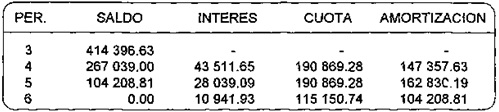
\includegraphics[height=3.0cm]{E7_9_1}
	\end{center}
	Segunda alternativa:
	\begin{center}
		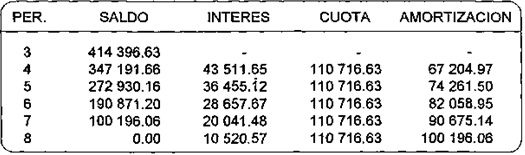
\includegraphics[height=4.0cm]{E7_9_2}
	\end{center}
	\medskip
	
	\item 10)	 Elaborar una tabla de capitalización para reunir la suma de \$350.000 en cuatro depósitos ordinarios de \$R c/u, más un depósito extraordinario de \$60.000, que se hará conjuntamente con el tercer depósito ordinario. Suponga una tasa del 9\% anual efectivo para el período.\\
	\textbf{ Respuesta:} \$62 233.1 
	\medskip
	
	\item 11)	 Elaborar una tabla, para que el día primero de septiembre de 1988 se hayan reunido \$500.000 en las siguientes condiciones:\\
	
	a)	depósitos semestrales ordinarios de \$R c/u; el primer depósito se efectuará el primero de marzo de 1986; el último depósito se efectuará el primero de septiembre de 1987; \\
	b)	se hará un depósito extraordinario de \$70.000 el primero de marzo de 1987;\\
	c)	tasa 30\% nasv Nominal anual semestre vencido.\\
	\textbf{Respuesta:}
	\begin{center}
		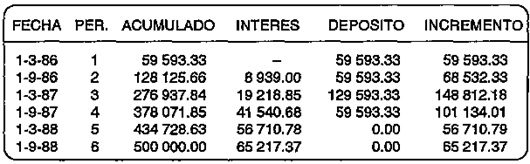
\includegraphics[height=4.0cm]{E7_11}
	\end{center}
	\medskip
	
	\item 12)	 Una deuda de \$2 millones está siendo amortizada mediante pagos mensuales uniformes, durante 15 años, con un interés del 27.6\% namv (Nominal anual mes vencido). Determinar qué parte del pago número 64 se utiliza a pagar intereses y cuánto a amortización.\\
	\textbf{ Respuesta:} intereses \$43.510.12; amortización, \$3.270.52
	\medskip
	
	\item 13)	 Se están reuniendo \$2 millones, mediante depósitos mensuales uniformes durante 5 años, en un fondo que paga el 30\% namv (Nominal anual mes vencido). Determinar cuál es el crecimiento del fondo, por concepto de intereses en el período 41. \\
	\textbf{Respuesta:} \$24.781.88
	\medskip
	
	\item 14)	 Una deuda de \$1.000 000 está siendo amortizada en pagos mensuales durante 15 años, con intereses al 30\% namv (Nominal anual mes vencido). Elaborar una tabla de amortización que muestre, únicamente, los períodos 108,109 y 110.\\
	\textbf{Respuesta:}
	\begin{center}
		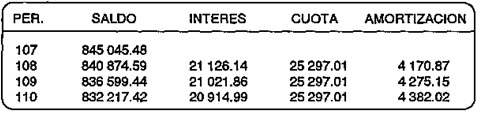
\includegraphics[height=3.5cm]{E7_14}
	\end{center}
	\medskip
	
	\item 15)	 Se está reuniendo un capital de \$1.000.000, mediante depósitos mensuales iguales durante 8 años en un fondo que paga el 30\% namv (Nominal anual mes vencido). Además, se ha acordado que, al momento de efectuar el depósito ordinario número 56, se hará un depósito extraordinario de \$70.000. Construir una tabla que muestre, únicamente los períodos 55, 56 y 57.\\
	\textbf{Respuesta:}
	\begin{center}
		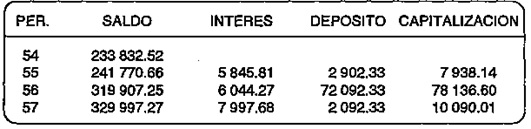
\includegraphics[height=4.0cm]{E7_15}
	\end{center}
	\medskip
	
	\item 16)	 Elaborar una tabla para amortizar la suma de \$600.000 en 6 pagos trimestrales, con cobro anticipado de intereses del 8.5\% ptv periódico  trimestral vencido y abonos vencidos e iguales a capital.
	\medskip
	
	\item Hallar el valor de la cuota total (intereses + amortización) que debe pagarse al final del mes 20 en una amortización de \$3 millones en pagos mensuales, durante 3 años, con cobro anticipado de intereses y abono a capital mensuales e iguales. Suponga una tasa del 2.5\% pma (periódico mensual anticipado).\\
	\textbf{Respuesta: }\$116 666.73
	\medskip
	
	\item 18)	 Hallar la primera cuota de amortización necesaria, para cancelar una deuda de \$100.000 en las siguientes condiciones:\\
	
	a) plazo de gracia muerto: 2 períodos; \\
	b) número de cuotas ordinarias: 4; \\
	c) cuota extraordinaria pactada de \$20.000, en el período 4 (coincide con el segundo pago ordinario); \\
	d) tasa 10\% anual efectiva para el período; \\
	e) característica de la cuota ordinaria:\\
	$e_{1}$)  Creciente lineal en \$6.000 \\
	$e_{2}$)  Decreciente lineal en -\$6.000\\
	\textbf{Respuestas:} $e_{1}$)  \$24 670.57;  $e_{2}$)  \$41 244.58
	\medskip
	
	\item 19) Hallar la primera cuota de amortización necesaria, para cancelar una deuda de \$100.000 en las siguientes condiciones:\\
	
	a)	plazo de gracia muerto: 2 períodos; \\
	b)	número de cuotas ordinarias: 4;\\
	c)	cuota extraordinaria pactada de \$20 000, en el período 4 (coincide con el segundo pago ordinario); \\
	d)	tasa 10\% anual efectiva para el período; \\
	e)	característica de la cuota ordinaria:\\
	$e_{1}$)  Creciente geométrica en 20\%\\
	$e_{2}$)  Decreciente geométrico en - 20\%\\
	\textbf{Respuestas: }$e_{1}$)  \$41 244.58;  $e_{2}$)  \$25 095.34\\
	\medskip
	
	\item 20)	 Elaborar una tabla en períodos anuales, que muestre la amortización de \$300.000 en 4 pagos, pero cada pago se efectúa cada 2 años y son crecientes en un 30\%. Suponga una tasa del 24\% efectivo anual.\\
	\textbf{Respuesta}
	\begin{center}
		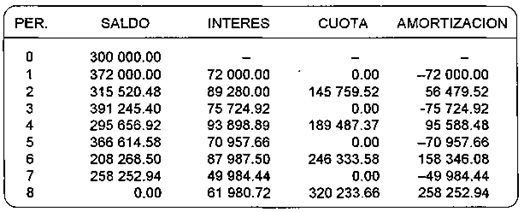
\includegraphics[height=4.0cm]{E7_20}
	\end{center}
	\medskip
	
	\item 21)Elaborar una tabla de amortización para cancelar una deuda de \$700.000 en 3 años mediante pagos semestrales bajo las siguientes condiciones: tasa de interés 28\% nasv (Nominal anual semestre vencido). dentro de cada año, el pago permanece constante pero; cada año:\\
	
	a.	el valor del pago aumenta un 20\% \\
	b.	el valor del pago disminuye un 20\% \\
	\textbf{Respuestas:}
	a)
	\begin{center}
		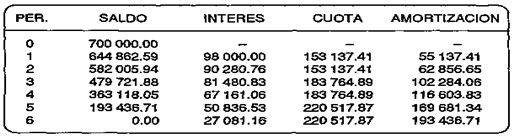
\includegraphics[height=4.0cm]{E7_21_1}
	\end{center}
	b)
	\begin{center}
		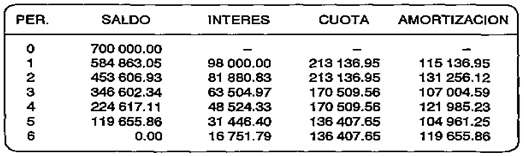
\includegraphics[height=4.0cm]{E7_21_2}
	\end{center}
	\medskip
	
	\item 22) Resuelva el problema anterior suponiendo que:\\
	
	a)	el pago global anual aumenta en \$15.000 (esto equivale a decir que: el valor de los pagos del gradiente aumentan en \$15.000 pero la diferencia entre las inter-cuotas no es de \$15.000) \\
	b)	el pago global anual disminuye en \$15.000\\
	\textbf{ Respuestas:}
	a)
	\begin{center}
		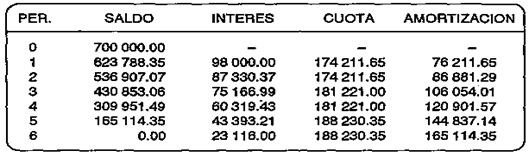
\includegraphics[height=4.0cm]{E7_22_1}
	\end{center}
	b)
	\begin{center}
		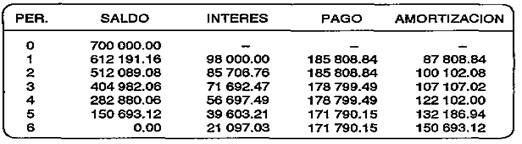
\includegraphics[height=4.0cm]{E7_22_2}
	\end{center}
	\medskip
	
	\item 23) Elaborar una tabla para amortizar la suma de \$900.000 en pagos semestrales durante 3 años, con la condición de aumentar cada año el valor de los pagos en \$60.000 pero dentro de cada año el valor de los pagos permanecen constantes. Utilice una tasa del 38\% nasv Nominal anual semestre vencido.\\
	\textbf{Respuesta:}\\
	\begin{center}
		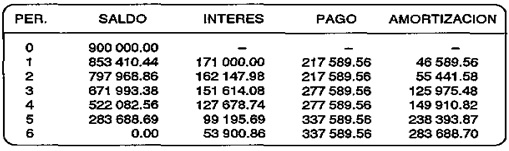
\includegraphics[height=4.0cm]{E7_23}
	\end{center}
	\medskip
	
	\item 24)	 Elaborar una tabla para amortizar la suma de \$800.000 en pagos semestrales durante 3 años, pero que crecen cada año en \$50.000, con una tasa del 42\% nasv (nominal semestre vencido).\\
	\textbf{Respuesta:}
	\begin{center}
		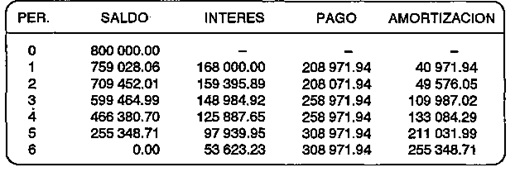
\includegraphics[height=4.0cm]{E7_24}
	\end{center}
	\medskip
	
	\item 25)	 Elaborar una tabla para amortizar la suma de \$100.000 en dos años, más un período de gracia muerto de 6 meses, con intereses al 30\% namv Nominal anual mes vencido., mediante pagos trimestrales iguales, pero con crecimiento anual de la cuota del 21\% (escalonado). Además, se efectuará un pago extraordinario de \$20.000, al final del mes 18.\\
	\textbf{Respuesta:}
	\begin{center}
		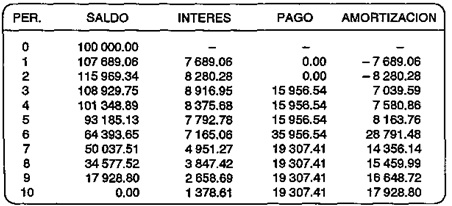
\includegraphics[height=4.0cm]{E7_25}
	\end{center}
	\medskip
	
	\item 26)	 Elaborar una tabla para capitalizar \$200.000 en 3 años, más un período de gracia de un año, mediante depósitos semestrales ordinarios que crezcan cada año un 25\%, pero dentro de cada año el valor de los depósitos es constante; además se efectuará un depósito extraordinario de \$40.000 en el período 3. Suponga un interés del 32\% nasv (nominal anual semestre vencido).\\
	\textbf{Respuesta:}
	\begin{center}
		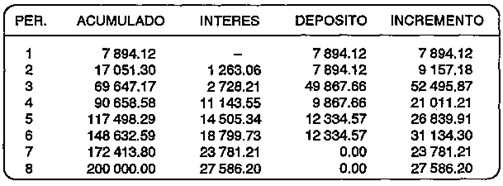
\includegraphics[height=4.0cm]{E7_26}
	\end{center}
	\medskip
	
	\item 27)	 Desea amortizarse la suma de \$5 millones, en cuotas mensuales, durante 20 años, con la condición de aumentar cada cuatro años la cuota mensual en un 50\%. Si suponemos una tasa del 32\% anual efectivo, calcular el valor del primero y del último pago. \\
	\textbf{Respuestas:} \$90.966.36 y \$460.517.19
	\medskip
	
	\item 28)	 Una deuda de \$2 millones está siendo amortizada en pagos mensuales, durante 15 años, con intereses al 30\% namv (nominal anual mes vencido) y crecimiento mensual de la cuota de \$300. Hallar la distribución del pago 105, entre intereses y abono a capital.\\
	\textbf{Respuesta:} intereses: \$66.323.59; amortización: \$4.111.98
	\medskip
	
	\item 29)	 Se está reuniendo la suma de \$5 millones mediante depósitos mensuales durante 8 años. Si los depósitos aumentan de valor cada mes \$200 y suponiendo un interés del 27\% namv (nominal anual mes vencido):\\
	
	a.	calcular el capital reunido hasta el período 63 \\
	b.	¿qué tanto del incremento al fondo en el período 64 es debido a intereses? \\
	\textbf{Respuestas: }a) \$1.840.961.97;  b) \$41.421.64
	\medskip
	
	\item 30)	 Una persona se compromete a cancelar una deuda de \$400.000, con intereses al 36\% naav (nominal anual trimestral vencido), mediante pagos trimestrales durante 10 años. Cada año, el valor de las cuotas crece un 15\%, pero dentro de cada año la cuota no varía. Determinar el valor de la cuota número 14, su distribución entre intereses y abono a capital y el saldo insoluto, inmediatamente después de haberse efectuado el pago número 14.\\
	\textbf{Respuestas:} valor de la cuota: \$39 942; 	intereses: \$48 590.21;
	Amortización: -\$8 648.22;       saldo: \$548 539.49\\
	\medskip
	\item 31)	 Una deuda de \$2 millones está siendo amortizada en pagos mensuales, durante 15 años, con la condición de incrementar la cuota cada año en un 18\% pero dentro de cada año la cuota permanece constante. Suponiendo un interés del 27\% namv (nominal anual mes vencido), determinar:\\
	
	a.	el valor del primer pago; \\
	b.	el valor del último pago; \\
	c.	 la deuda, inmediatamente después de haber efectuado el pago 1 00; \\
	d.	la distribución del pago 101. \\
	\textbf{Respuestas: }a) \$23 706.16;	 b) \$240 552.22; 	e) \$4 976 930.72; 
	d) interés: \$111 980.94, amortización: - \$22 872.81
	\medskip
	
	\item 32)	 Elaborar una tabla para amortizar la suma de \$700.000, en pagos semestrales, con las siguientes condiciones:\\
	
	a.	el primer año se otorga, como período de gracia muerto (significa que no hay pagos y los intereses que se causan se abonan a capital)\\
	b.	el segundo año se otorga como período de gracia con cuota reducida( significa que solo, se pagan intereses pero no hay abono a capital) \\
	c.	en los siguientes 2 años se efectuarán pagos semestrales ordinarios crecientes en un 15\% \\
	d.	debe incluirse una cuota extra de \$50.000 en el período 6 (la cuota extra coincide con el segundo pago ordinario) \\
	e.	tasa de interés: 30\% nasv (nominal anual semestre vencido).\\
	
	\textbf{ Respuesta:}
	\begin{center}
		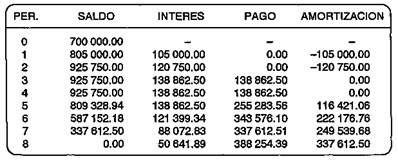
\includegraphics[height=4.0cm]{E7_32}
	\end{center}
	\medskip
	
	\item 33)	 Resolver el problema anterior, suponiendo que el crecimiento es escalonado anual del 15\%. \\
	\textbf{Respuesta:}
	\begin{center}
		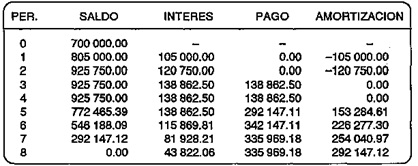
\includegraphics[height=4.0cm]{E7_33}
	\end{center}
	\medskip
	
	\item 34) Elaborar una tabla para amortizar la suma de \$800.000, en valor constante, mediante pagos trimestrales, durante 15 meses, suponiendo un interés del 30\% naav (nominal anual trimestre vencido) y que el índice de corrección monetaria permanecerá constante en el 8\% pmv (Periódico trimestral vencido).\\
	\textbf{ Respuesta:}
	\begin{center}
		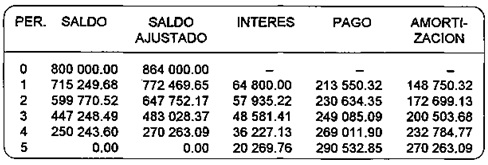
\includegraphics[height=4.0cm]{E7_34}
	\end{center}
	\medskip
	
	\item 35)   Elaborar una tabla para amortizar la suma de \$600.000, en cuatro pagos trimestrales decrecientes en \$50.000; pero en valor constante, utilice un interés del 8\% naav (nominal anual trimestre vencido) y suponga que la tasa de corrección monetaria permanecerá constante en el 22\% naav (nominal anual trimestre vencido). 
	\textbf{Respuesta:}
	\begin{center}
		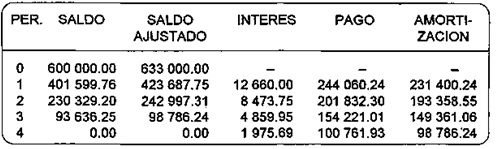
\includegraphics[height=4.0cm]{E7_35}
	\end{center}
	\medskip
	
	\item 36) Elaborar una tabla para amortizar en valor constante la suma de \$600.000, en 3 pagos anuales que decrecen anualmente en un 20\%. Suponga que la corrección monetaria permanece constante en el 22\% anual  efectivo y que se cobra un interés del 10\% anual  efectivo. \\
	\textbf{Respuesta}
	\begin{center}
		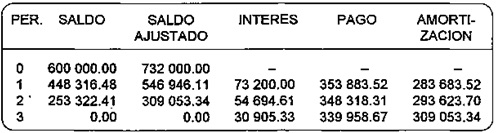
\includegraphics[height=4.0cm]{E7_36}
	\end{center}
	\medskip
	
	\item  37) Suponga que en el problema anterior el gradiente es escalonado, con pagos semestrales.\\
	
	\textbf{ Respuesta:}
	\begin{center}
		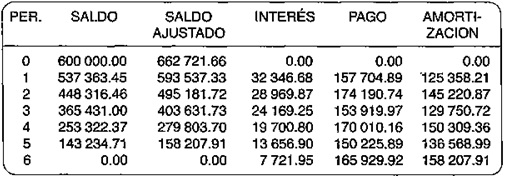
\includegraphics[height=4.0cm]{E7_37}
	\end{center}
	\medskip
	
	\item 38)  Un préstamo por valor de \$3 millones a 15 años con una tasa del 2.75\% pmv (periódico mes vencido) va ser amortizado en pagos mensuales durante 15 años con la condición de aumentar anualmente la cuota mensual en un 18\% durante los primeros 8 años y de ahí en adelante las cuotas mensuales crecerán anualmente en un 12\%. Calcular el valor de las cuotas durante el primer año y el valor da las cuotas durante el noveno año. \\
	\textbf{Respuestas:} cuota mensual primer año \$49 900.69; 
	Cuota mensual noveno año \$178 032.24
	\medskip
	
	\item 39)  Elaborar una tabla para amortizar la suma de \$12 millones si el crédito es concedido por una entidad financiera que cobra la tasa Libor + 8 puntos, para ser pagado en cuatro cuotas trimestrales vencidas en dólares. Al momento de otorgar el crédito se conoce la siguiente información: \\
	
	a.	Cambio US\$1 = \$3.000 \\
	b.	Tasa de devaluación proyectada 7\% EA, se asume que la devaluación es uniforme a través del año. \\
	c.	Tasa Libor = 2\% EA, se presume que no va a variar. \\
	
	Elabore una tabla que como mínimo muestre, en pesos, el saldo y el pago. Trabajar cualquier tasa con 5 decimales.\\ 
	Recuerde que cuando sume dos tasas efectivas debe usar la tasa    combinada.\\
	
	\textbf{ Respuesta:}
	\begin{center}
		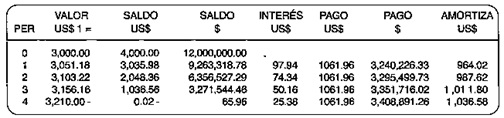
\includegraphics[height=4.0cm]{E7_39}
	\end{center}
	\medskip
	
	\item 40)  Elaborar una tabla para amortizar la suma de \$3 millones a la tasa del 18\% nasv (nominal anual semestre vencido) a un plazo de 3 años con cuotas semestrales por el sistema de abonos pactados a capital.\\
	
	Se ha pactado que en cada uno de los semestres 1 y 2 se amortiza el 1 0\% de la deuda.\\
	En cada uno de los semestres 3 y 4 se amortiza el 20\% de la deuda. \\
	En cada uno de los semestres 5 y 6 se amortiza el 25\% de la deuda.\\
	
	\textbf{Respuesta parcial:} el valor de los pagos será: \$270.000, 243.000, 216.000, 175.500, 135.000, 67.500
	\medskip
	
	\item 41)  Elaborar una tabla para amortizar la suma de \$4 millones en pagos trimestrales durante un año por el sistema de cuota fija con tasa variable. Tasa de interés DTF + 14 puntos. \\
	
	En el momento de otorgar el crédito la DTF = 7.5\% NTA.\\
	
	A los 3 meses la DTF = 7.7\% NTA\\ 
	A los 6 meses la DTF = 7.9\% NTA \\
	A los 3 meses la DTF = 8.3\% NTA \\
	A los 3 meses la DTF = 7.8\% NTA\\
	Trabajar las tasa con 5 decimales\\
	\textbf{Respuesta parcial:} Cuota fija \$1.145.927.48, valor del último pago \$1 158.346.26.
	\medskip
	
	\item 42)  Una empresa necesita cambiar de vehículo cada 3 años dando en parte de pago el vehículo usado y el resto se cancelará al contado con dineros provenientes de un fondo que paga el 33\% namv nominal anual mes vencido. Calcular el valor del depósito mensual uniforme necesario suponiendo las siguientes condiciones: \\
	
	a.	el precio actual, del vehículo nuevo es de \$6 millones y cada 3 meses aumenta de precio un 4.8\%. 
	b.	el vehículo, que se compre actualmente, a pesar de su uso y debido a procesos inflacionarios sube de precio cada 3 meses a razón del 3.2\%.\\
	\textbf{Respuesta:} \$29.491.33
	\medskip
	
	\item 43) Suponga que en el ejemplo anterior el fondo paga el 32\% naav nominal anual trimestre vencido y se constituye mediante depósitos trimestrales crecientes en un 8\%. Hallar el depósito en el fondo del primero y del último trimestre.\\
	\textbf{Respuestas:} \$63.452.34 y \$147.947.94
	\medskip
	
	\item 44)  Actualmente se contrae una deuda de \$600.000 para ser cancelada al final de 2 años y mientras tanto se deberá pagar un interés del 40\% naav nominal anual trimestre vencido. A fin de dar cumplimiento al pago de la deuda en su debida oportunidad se constituye un fondo de amortización que paga el 36\% naav nominal anual trimestre vencido mediante depósitos trimestrales iguales. \\
	
	a.	calcular el costo trimestral de la deuda.\\
	b.	si en lugar de constituir el fondo de amortización se hace una amortización usando como cuota de amortización el costo trimestral de la deuda. ¿A qué tasa nominal capitalizable trimestralmente se estaría amortizando la deuda?\\
	\textbf{Respuestas:} a) \$114.404.13 b) 41.89\% naav nominal anual trimestre vencido.
	\medskip
	
	\item 45) En el problema anterior. ¿Qué tanto del incremento al fondo en el período 7 es debido a intereses? \\
	\textbf{Respuesta:}\$36.837.38
	\medskip
	
	\item 46) Elabore una tabla para el fondo.
	\medskip
	
	\item 47) Una persona deposita \$1 000 000 en un fondo de amortización que paga el 21\% namv (nominal anual mes vencido). Un año después comenzó a depositar en la misma cuenta \$20.000 mensuales. ¿Cuánto tiempo tendrá que esperar para completar como mínimo \$2.000.000? \\
	\textbf{Respuesta:} 29 meses.
	\medskip
	
	\item 48) Una persona depositó \$10.000 trimestrales en un fondo de capitalización que pagaba el 28\% naav (nominal anual trimestre vencido).  Estos depósitos los hizo durante 5 años. A partir de ahí comenzó a retirar por semestre vencido la suma de \$50.000. ¿Durante cuánto tiempo podrá retirar? \\
	\textbf{Respuesta:} infinitos retiros
	\medskip
	
	\item 49) Usted desea capitalizar \$10 millones. Para eso abre una cuenta hoy con \$100.000 en un fondo de capitalización que paga el 2\% pmv (Periódico mensual vencido) y piensa depositar en esa cuenta \$5.000 al final de cada mes. ¿Cuánto tiempo tendrá que estar haciendo estos abonos para que como mínimo alcance la meta que se propone? \\
	\textbf{Respuesta: }171 meses
	\medskip
	
	\item 50) Una deuda de \$1.000.000 con intereses al 20\% nasv (nominal anual semestre vencido), se va a cancelar en pagos semestrales vencidos durante 10 años. Inmediatamente después de efectuar el pago 12 deudor y acreedor acuerdan suspender los pagos semestrales y cancelar el saldo de la deuda de un solo contado a su vencimiento con sus respectivos intereses. Para dar cumplimiento al pago se constituye un fondo de amortización mediante depósitos mensuales iguales que ganan un interés del 2.8\% pmv (Periódico mensual vencido). \\
	
	a.	¿Cuáles son los derechos del deudor y acreedor inmediatamente después del pago 12? \\
	b.	¿Cuál debe ser el valor de los depósitos en el fondo?\\
	\textbf{Respuestas:} a) deudor \$373.361.60; acreedor \$626.638.40; b) \$13.606.66
	
\end{itemize}